\chapter{The Nondeterministic Constraint Logic (NCL)} \label{chap:NCL}
In this Chapter, the Nondeterministic Constraint Logic model of computation is presented. This framework developped by Demaine and Hearn is
motivated by the Sliding-block puzzles \cite{hordern_sliding_1986}. The main result of \cite{hearn_pspace-completeness_2004} introduces the new
nondeterministic model of computation based on reversing edge directions in weighted directed graphs with minimum in-flow constraints on vertices.
This model, referred to as Nondeterministic Constraint Logic, or NCL, is shown to have the same computational power as a space-bounded Turing machine.

Several decision problems surrounding the NCL framework are proved to be $\PSPACE$-complete \cite{hearn_pspace-completeness_2004}. These decision problems are then used to prove the
$\PSPACE$-completeness of well-known Sliding-block puzzles such as Rush Hour and Sokoban \cite{hearn_demaine_ncl_book}. Demaine and Hearn argue that NCL can be considered as a
model of computation in its own right instead of just a set of decision problems. Thus, proving a problem to be $\PSPACE$-hard in the NCL
framework simply requires the construction of a couple of gadgets that can be connected together.
In the last section of \cite{hearn_pspace-completeness_2004} gives an interesting equivalent formulation of NCL in terms of sliding tokens along
graph edges. This latter formulation will be the focus of sections \ref{sec:sliding_tokens} and \ref{sec:labeled_sliding_token} to prove that
the Sliding token problem and labelled variant of the sliding token problem are $\PSPACE$-complete (theorems \ref{theorem:ncl_sliding_token}
and \ref{theorem:labeled_sliding} respectively).

\textit{Roadmap.} Section \ref{sec:formalism} describes the constraint logic using a graph formulation.
Section \ref{sec:contraint_graph} gives an overview of AND/OR constraint graphs which is the primary formulation used in the NCL framework.
Section \ref{sec:ncl_results} present some complexity results of decision problems stemming from the constraint logic framework.
In section \ref{sec:sliding_tokens} we detail the $\PSPACE$-completeness proof of the sliding token problem using the alternative
formulation of NCL (theorem \ref{theorem:ncl_sliding_token}). Lastly, in section \ref{sec:labeled_sliding_token} the hardness proof of the
labeled variant of the sliding token problem is given.

\section{Graph Formulation}\label{sec:formalism}
An NCL machine consists of a \textit{constraint graph}, $G = (V,E)$ that we can think of as our computation model.
Let $G$ be a $3$-regular graph with edge weights $ \in \{1, 2\}$. An edge is then called \textit{red} or \textit{blue}, respectively.
Each vertex has a nonnegative \textit{minimum inflow} which is the sum of the weights on inward-directed edges. A \textit{legal configuration}
is an assignment of an \textit{orientation(direction)} to each edge such that for every vertex $v$ of $G$, the sum of weights of inward-directed
edges of $v$ is at least $2$. A \textit{legal move} is the reversal of a single edge that results in another legal configuration.


\section{AND/OR Constraint Graphs} \label{sec:contraint_graph}
As part of the constraint logic framework,  Hearn and Demaine provided a restricted variant of Nondeterministic Constraint Logic (restricted NCL),
in which the constraint graph $G$ is planar, $3$-regular, uses only weights $ \in \{1,2\}$ and the graph is constructed from only two specific vertex
types ($AND$ and $OR$ vertices). A vertex $v$ of $G$ is an \textit{AND vertex} if exactly one incident edge has weight $2$ (Figure \ref{fig:and_vertex}) and
a vertex $v$ of $G$ is an \textit{OR vertex} if all the incident edges have weight $2$ (Figure \ref{fig:or_vertex}). Thus, a graph
$G$ is an \textit{AND/OR constraint graph} if it consists of only $AND$ and $OR$ vertices.

%%%%%%%%%%%%%%%%%%%%%%%%%%%%%% BEGINING OF A FIGURE : AND and OR vertex of constraint graph %%%%%%%%%%%%%%%%%%%%%%%%%%%%%
\begin{figure}[H]
  \begin{subfigure}[b]{0.4\textwidth}
    \centering
      \begin{scaletikzpicturetowidth}{\textwidth}
        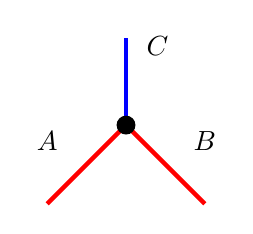
\begin{tikzpicture}
          \def\xa{0}     % AND
          \def\ya{0}
          %labels
          \node (1) at (\xa+0.4,\ya+1) {$C$};
          \node (2) at (\xa+1,\ya-0.2) {$B$};
          \node (2) at (\xa-1,\ya-0.2) {$A$};
          % f_1 arrows
          \draw[ultra thick, -, blue] (\xa, \ya) -- (\xa, \ya+1.1);
          \draw[ultra thick, -, red] (\xa, \ya) -- (\xa+1, \ya-1);
          \draw[ultra thick, -, red] (\xa, \ya) -- (\xa-1, \ya-1);
          % Nodes fill
          \path[fill] (\xa,\ya) circle (\ver);
        \end{tikzpicture}
      \end{scaletikzpicturetowidth}
      \caption{And vertex. Edge $C$ may be directed outward if and only if edges $A$ and $B$ are both directed inward.}
      \label{fig:and_vertex}
  \end{subfigure}
  \hspace{5em} % vertical space
  \begin{subfigure}[b]{0.4\textwidth}
    \centering
    \begin{scaletikzpicturetowidth}{\textwidth}
      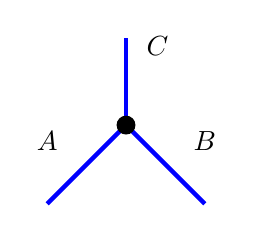
\begin{tikzpicture}
        \def\xb{5} % OR
        \def\yb{0}
        %labels
        \node (1) at (\xb+0.4,\yb+1) {$C$};
        \node (2) at (\xb+1,\yb-0.2) {$B$};
        \node (2) at (\xb-1,\yb-0.2) {$A$};
        % f_2 arrows
        \draw[ultra thick, -, blue] (\xb, \yb) --(\xb, \yb+1.1);
        \draw[ultra thick, -, blue] (\xb, \yb) --(\xb+1, \yb-1);
        \draw[ultra thick, -, blue] (\xb, \yb) --(\xb-1, \yb-1);
        % Nodes fill
        \path[fill] (\xb,\yb) circle (\ver);     % OR
      \end{tikzpicture}
    \end{scaletikzpicturetowidth}
    \caption{Or vertex. Edge $C$ may be directed outward if and only if either edge $A$ or edge $B$ is directed inward.}
    \label{fig:or_vertex}
  \end{subfigure}
  \caption{And and Or vertices. Red edges have weight $1$, blue edges have weight $2$, and all vertices have a minimum in-flow constraint of $2$.}
  \label{fig:and_or_vertices}
\end{figure}
%%%%%%%%%%%%%%%%%%%%%%%%%%%%%%%%%%%%%%%% ENDING OF A FIGURE %%%%%%%%%%%%%%%%%%%%%%%%%%%%%%%%%

\section{NCL Results} \label{sec:ncl_results}
This section compiles the important complexity results linked to NCL. A first fundamental decision problem that arises in the NCL framework
is about the satisfiability of a given constraint graph $G$. It is defined as follows :
\begin{flushleft}
  CONSTRAINT GRAPH SATISFIABILITY \\
  \textbf{Instance: } A constraint graph $G$. \\
  \textbf{Question: } Does $G$ have a legal configuration ? \\
\end{flushleft}
In \cite{hearn_demaine_ncl_book} Demaine and Hearn proved that the CONSTRAINT GRAPH SATISFIABILITY problem is $\NP-$complete.

Another important problem regarding constraint graphs is about their reconfigurability. The CONFIGURATION-TO-CONFIGURATION (C2C) problem asks
if given two configurations of a constraint graph $G$, whether they can be reconfigured into each other.
\begin{flushleft}
  CONFIGURATION-TO-CONFIGURATION (C2C)\\
  \textbf{Instance: } A constraint graph $G$ and two legal configurations $C_1, C_2$ for $G$. \\
  \textbf{Question: } Is there a sequence of legal configurations from $C_0, C_1, \dots , C_t$ such that $C_i$ is obtained from $C_{i-1}$
  by a legal move for each $i$ with $1 \leq i \leq t$ and $C_0 = C_1, C_t = C_2$ ? \\
\end{flushleft}
Hearn and Demaine established that the C2C problem is $\PSPACE$-complete\cite{hearn_demaine_ncl_book}.

Similar to the C2C problem, the CONFIGURATION-TO-EDGE (C2E) problem asks whether a target edge $e$ can be reversed
given a constraint graph $G$.
\begin{flushleft}
  CONFIGURATION-TO-EDGE (C2E) \\
  \textbf{Instance: } A constraint graph $G$, a target edge $e$ from $G$ and an initial legal configuration $C$ for $G$ . \\
  \textbf{Question: } Is there a sequence of legal configurations, starting with $C$, where every configuration is obtained from the previous
  by changing the orientation of one edge, so that $e$ is eventually reversed? \\
\end{flushleft}
Hearn and Demaine proved that the C2E problem is also $\PSPACE$-complete\cite{hearn_demaine_ncl_book}.

More interestingly, the hardness result for C2C and C2E still holds when the vertices of $G$ are restricted to be $AND$ and $OR$ vertices
defined in section \ref{sec:contraint_graph} ans referred as restricted NCL. C2C and C2E hardness proof involves a reduction from quantified
Boolean formulas, based on the logical interpretation of AND/OR constraint graphs. Additional gadgets are required for simulating quantifiers
and for converting red edges into blue edges (and vice versa), which can all be accomplished by combinations of $AND$ and $OR$
vertices \cite{hearn_demaine_ncl_book}.

Demaine and Hearn in fact strengthen this result even further and show that C2C and C2E both remain $\PSPACE$-complete when the constraint
graph $G$ is planar \cite{hearn_demaine_ncl_book}. This proof involves the construction of crossover gadgets that allow two edges to cross
each other.

It is also possible to impose an additional restriction, while preserving the hardness of these problems: each vertex with three blue edges
can be required to be part of a triangle with a red edge. Such a vertex is called a protected or, and it has the property that
(in any valid orientation of the whole graph) it is not possible for both of the blue edges in the triangle to be directed inwards.
This restriction makes it easier to simulate these vertices in hardness reductions for other problems\cite{hearn_demaine_ncl_book}.
Additionally, the constraint graphs can be required to have bounded bandwidth, and the problems on them will still remain
$\PSPACE$-complete\cite{van_der_zanden_parameterized_nodate}.


\section{Alternative formulation : Sliding tokens} \label{sec:sliding_tokens}
The SLIDING TOKEN problem was introduced by Hearn and Demaine in \cite{hearn_pspace-completeness_2004} as a variant of SLIDING-BLOCK puzzle
with $1 \times 1 $ blocks on a graph but require no adjacent tokens, which can be seen as a reconfiguration problem for Independent Set.
Suppose that we are given two independent sets $I_b$ and $I_r$ of a graph $G =(V,E)$ such that $|I_b| = |I_r|$ and imagine that a
\textit{token} is placed on each vertex in $I_b$. Then, the SLIDING TOKEN problem is to determine whether there exists a sequence
$ S = \langle I_1, I_2, \dots, I_l \rangle$ of independent sets of $G$ such that :
\begin{enumerate}
  \item $I_1 = I_b, I_l = I_r,$ and $|I_i| = |I_b| = |I_r|$ for all $i, 1 \leq i \leq l;$ and
  \item For each $i, 2 \leq i \leq l$ there is an edge $xy$ in $G$ such that  $I_{i-1} \setminus I_{i} = \{x\}$ and $I_{i} \setminus I_{i-1} = \{y\}$.
\end{enumerate}
That is, $I_i$ can be obtained from $I_{i-1}$ by sliding exactly one token on a vertex $x \in I_{i-1}$ to its adjacent vertex $y \in I_{i}$
along an edge $xy \in E(G)$. Such a sequence $S$, if exists, is called a \textit{TS-sequence} in $G$ between $I_b$ and $I_r$.
We denote by a $3$-tuple $(G, I_{b}, I_{r})$ an instance of SLIDING TOKEN problem.  If a TS-sequence $S$ in $G$ between $I_{b}$ and $I_{r}$ exists,
we say that $I_{b}$ is \textit{reconfigurable} to $I_{r}$ (and vice versa), and write $I_{b} \overset{G}\leftrightsquigarrow I_{r}$. The sets
$I_{b}$ and $I_{r}$ are the \textit{initial} and \textit{target} independent sets, respectively. For a TS-sequence $S$, the \textit{length}
len($S$)of $S$ is defined as the number of independent sets in $S$ minus one. In other words, len($S$) is the number of \textit{token-slides}
described in $S$. Figure \ref{fig:sliding_token_example} illustrates a TS-sequence of length $4$ between two independent sets
$I_{b} = I_{1}$ and $I_{r} = I_{5}$.

\begin{figure}[H]
  \centering
    \begin{scaletikzpicturetowidth}{\textwidth}
      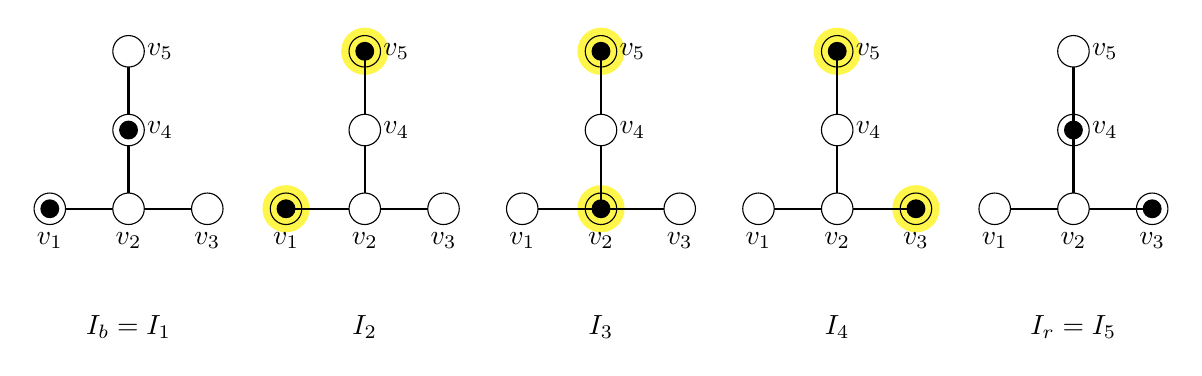
\begin{tikzpicture}[scale=1]
        \def\x{1}
        \def\xa{0}
        \def\ya{0}
        \def\xb{3}
        \def\xc{6}
        \def\xd{9}
        \def\xe{12}

        %graph G
        %edges
        \draw[thick] (\xa,\ya)--(\xa+1,\ya)--(\xa+1,\ya+1)--(\xa+1,\ya+2);
        \draw[thick] (\xa+1,\ya)--(\xa+2,\ya);
        %nodes
        \draw[fill=white] (\xa,\ya) circle (0.2cm);     %v1
        \draw[fill=white] (\xa+1,\ya+1) circle (0.2cm); %v2
        \draw[fill=white] (\xa+1,\ya+2) circle (0.2cm); %v3
        \draw[fill=white] (\xa+2,\ya) circle (0.2cm);   %v4
        \draw[fill=white] (\xa+1,\ya) circle (0.2cm);   %v5
        % Tokens
        \path[fill] (\xa+1,\ya+1) circle (\ver);
        \path[fill] (\xa,\ya) circle (\ver);
        %labels
        \node (1) at (\xa,\ya-0.4) {$v_1$};
        \node (2) at (\xa+1+0.4,\ya+1) {$v_4$};
        \node (3) at (\xa+1+0.4,\ya+2) {$v_5$};
        \node (5) at (\xa+2,\ya-0.4) {$v_3$};
        \node (4) at (\xa+1,\ya-0.4) {$v_2$};
        \node (1) at (\xa+1,\ya-1.5) {$I_b = I_1$};

        %G_1
        % Highlights
        \draw[fill=yellow, opacity=.7, draw=none] (\xb+1,\ya+2) circle (0.3cm);
        \draw[fill=yellow, opacity=.7, draw=none] (\xb,\ya)  circle (0.3cm);
        %edges
        \draw[thick] (\xb,\ya)--(\xb+1,\ya)--(\xb+1,\ya+1)--(\xb+1,\ya+2);
        \draw[thick] (\xb+1,\ya)--(\xb+2,\ya);
        %nodes
        \draw             (\xb,\ya) circle (0.2cm);    %v1
        \draw[fill=white] (\xb+1,\ya+1) circle (0.2cm);%v2
        \draw             (\xb+1,\ya+2) circle (0.2cm);%v3
        \draw[fill=white] (\xb+2,\ya) circle (0.2cm);  %v4
        \draw[fill=white] (\xb+1,\ya) circle (0.2cm);  %v5
        % Tokens
        \path[fill] (\xb+1,\ya+2) circle (\ver);
        \path[fill] (\xb,\ya) circle (\ver);
        %labels
        \node (1) at (\xb,\ya-0.4) {$v_1$};
        \node (2) at (\xb+1+0.4,\ya+1) {$v_4$};
        \node (3) at (\xb+1+0.4,\ya+2) {$v_5$};
        \node (5) at (\xb+2,\ya-0.4) {$v_3$};
        \node (4) at (\xb+1,\ya-0.4) {$v_2$};
        \node (1) at (\xb+1,\ya-1.5) {$I_2$};

        %G_2
        % Highlights
        \draw[fill=yellow, opacity=.7, draw=none] (\xc+1,\ya+2) circle (0.3cm);
        \draw[fill=yellow, opacity=.7, draw=none] (\xc+1,\ya)  circle (0.3cm);
        %edges
        \draw[thick] (\xc,\ya)--(\xc+1,\ya)--(\xc+1,\ya+1)--(\xc+1,\ya+2);
        \draw[thick] (\xc+1,\ya)--(\xc+2,\ya);
        %nodes
        \draw[fill=white] (\xc,\ya) circle (0.2cm);    %v1
        \draw[fill=white] (\xc+1,\ya+1) circle (0.2cm);%v2
        \draw             (\xc+1,\ya+2) circle (0.2cm);%v3
        \draw[fill=white] (\xc+2,\ya) circle (0.2cm);  %v4
        \draw             (\xc+1,\ya) circle (0.2cm);  %v5
        % Tokens
        \path[fill] (\xc+1,\ya+2) circle (\ver);
        \path[fill] (\xc+1,\ya)  circle (\ver);
        %labels
        \node (1) at (\xc,\ya-0.4) {$v_1$};
        \node (2) at (\xc+1+0.4,\ya+1) {$v_4$};
        \node (3) at (\xc+1+0.4,\ya+2) {$v_5$};
        \node (5) at (\xc+2,\ya-0.4) {$v_3$};
        \node (4) at (\xc+1,\ya-0.4) {$v_2$};
        \node (1) at (\xc+1,\ya-1.5) {$I_3$};

        %G_3
        % Highlights
        \draw[fill=yellow, opacity=.7, draw=none] (\xd+1,\ya+2) circle (0.3cm);
        \draw[fill=yellow, opacity=.7, draw=none] (\xd+2,\ya)  circle (0.3cm);
        %edges
        \draw[thick] (\xd,\ya)--(\xd+1,\ya)--(\xd+1,\ya+1)--(\xd+1,\ya+2);
        \draw[thick] (\xd+1,\ya)--(\xd+2,\ya);
        %nodes
        \draw[fill=white] (\xd,\ya) circle (0.2cm);    %v1
        \draw[fill=white] (\xd+1,\ya+1) circle (0.2cm);%v2
        \draw             (\xd+1,\ya+2) circle (0.2cm);%v3
        \draw             (\xd+2,\ya) circle (0.2cm);  %v4
        \draw[fill=white] (\xd+1,\ya) circle (0.2cm);  %v5
        % Tokens
        \path[fill] (\xd+1,\ya+2)  circle (\ver);
        \path[fill] (\xd+2,\ya) circle (\ver);
        %labels
        \node (1) at (\xd,\ya-0.4) {$v_1$};
        \node (2) at (\xd+1+0.4,\ya+1) {$v_4$};
        \node (3) at (\xd+1+0.4,\ya+2) {$v_5$};
        \node (5) at (\xd+2,\ya-0.4) {$v_3$};
        \node (4) at (\xd+1,\ya-0.4) {$v_2$};
        \node (1) at (\xd+1,\ya-1.5) {$I_4$};

        %G4
        %edges
        \draw[thick] (\xe,\ya)--(\xe+1,\ya)--(\xe+1,\ya+1)--(\xe+1,\ya+2);
        \draw[thick] (\xe+1,\ya)--(\xe+2,\ya);
        %nodes
        \draw[fill=white] (\xe,\ya) circle (0.2cm);    %v1
        \draw             (\xe+1,\ya+1) circle (0.2cm);%v2
        \draw[fill=white] (\xe+1,\ya+2) circle (0.2cm);%v3
        \draw             (\xe+2,\ya) circle (0.2cm);  %v4
        \draw[fill=white] (\xe+1,\ya) circle (0.2cm);  %v5
        % Tokens
        \path[fill] (\xe+1,\ya+1)  circle (\ver);
        \path[fill] (\xe+2,\ya) circle (\ver);
        %labels
        \node (1) at (\xe,\ya-0.4) {$v_1$};
        \node (2) at (\xe+1+0.4,\ya+1) {$v_4$};
        \node (3) at (\xe+1+0.4,\ya+2) {$v_5$};
        \node (5) at (\xe+2,\ya-0.4) {$v_3$};
        \node (4) at (\xe+1,\ya-0.4) {$v_2$};
        \node (1) at (\xe+1,\ya-1.5) {$I_r = I_5$};
      \end{tikzpicture}
    \end{scaletikzpicturetowidth}
  \caption{TS sequence $ \langle I_1, I_2,\dots,I_5 \rangle$ of independent sets which transforms $I_b = I_1$ into $I_r = I_5$ where the vertices in independent sets are depicted by small black circles (tokens).}
  \label{fig:sliding_token_example}
\end{figure}

\subsection{Known results for the SLIDING TOKEN problem.}
Analogous to the Independent Set problem being the key problem among thousands of $\NP$-complete problems to prove $\NP$-hardness,
the SLIDING TOKEN problem plays an important role since several $\PSPACE$-hardness results have been proved using reductions from it.

For the sliding token problem, some polynomial time algorithms have been investigated as follows: Linear time algorithms have been shown
for cographs (also known as P4-free graphs) \cite{kaminski_complexity_2012} and trees \cite{2014arXiv1406.6576D}. Polynomial time algorithms
are shown for bipartite permutation graphs \cite{fox-epstein_sliding_2015}, and claw-free graphs \cite{bonsma_reconfiguring_2014}.
On the other hand, $\PSPACE$-completeness is shown for graphs of bounded treewidth \cite{mouawad_reconfiguration_2014}, and planar
graphs \cite{hearn_pspace-completeness_2004}.

\subsection{$\PSPACE$-completeness.}

In this section we go over the $\PSPACE$-completeness result of the SLIDING TOKEN problem, proved by a reduction from NCL. As seen in
section \ref{sec:ncl_results}, there are slightly different versions of decision problems for NCL and all of them are $\PSPACE-$complete.
For our purpose, we just need the version for the configuration-to-configuration for planar NCL. Recall that an instance of the
C2C planar NCL problem is defined on a $3-$regular, planar, directed graph where each edge has a weight $\in \{1,2\}$ and each vertex is
either and $AND$ or an $OR$ vertex. The proof of theorem \ref{theorem:ncl_sliding_token} is organised in sections
\ref{subsubsection:reduction_structure} to \ref{subsubsection:and_or} which explains the reduction structure, gadets used and how they are
connected together.

\subsubsection{Reduction structure.}\label{subsubsection:reduction_structure}
To show that the SLIDING TOKEN problem is $\PSPACE$-complete we provide a reduction from configuration-to-configuration for AND/OR graphs
such that the NCL instance is solvable if and only if the corresponding SLIDING TOKEN is solvable. The sliding token instance is constructed by
piecing together gadgets which emulates the directed edges, the AND vertices and the OR vertices of the given NCL instance.
We construct the corresponding NCL $AND$ and $OR$ vertex gadgets out of sliding-token subgraphs illustrated in figures
\ref{fig:and_gadget_sliding_token} and \ref{fig:or_gadget_sliding_token} respectively.

\subsubsection{The OR gadget and the AND gadget.}\label{subsubsection:or_and}
The construction of Fig.\ref{fig:and_gadget_sliding_token} satisfies the same constraints as an NCL $AND$ vertex, with the upper
token corresponding to the blue edge and both lower tokens corresponding to the red edges. The upper token can slide in only when both lower
tokens are slid out thus maintaining the flow constraint of an NCL AND vertex.
Likewise, the construction of Fig.\ref{fig:or_gadget_sliding_token} satisfies the same constraints as an NCL $OR$ vertex with the upper
and two lower tokens corresponding the the $OR$ blue edges. The upper token in the $OR$ gadget can slide in when  either lower token is slid
out and the internal token can then slide to one side or the other to make room. Here it is the internal token that ensures the NCL flow
constraint is satisfied by sliding on a appropriate vertex among the three internal nodes to force one among the outer tokens are slid in.

%%%%%%%%%%%%%%%%%%%%%%%%%%%%%%%%%%%%%%%%%%%% BEGINING OF A FIGURE : AND and OR gadget of Sliding Token %%%%%%%%%%%%%%%%%%%%%%%%%%%%%%%%%%%%
\begin{figure} [H]
  \begin{subfigure}[b]{0.4\textwidth}
    \centering
    \begin{scaletikzpicturetowidth}{\textwidth}
      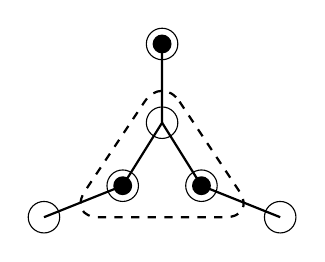
\begin{tikzpicture}
        \def\xa{0}
        \def\ya{0}
        %graph G
        \draw (\xa,\ya) circle (0.2cm);          %v1 no fill
        \draw (\xa,\ya+1) circle (0.2cm);        %v2 no fill
        \draw (\xa+0.5,\ya-0.8) circle (0.2cm);  %v4 no fill
        \draw (\xa-0.5,\ya-0.8) circle (0.2cm);  %v3 no fill
        \draw (\xa-1.5,\ya-1.2) circle (0.2cm);  %v5 no fill
        \draw (\xa+1.5,\ya-1.2) circle (0.2cm);  %v6 no fill
        \path[fill] (\xa,\ya+1) circle (\ver);       %v2
        \path[fill] (\xa+0.5,\ya-0.8) circle (\ver); %v4
        \path[fill] (\xa-0.5,\ya-0.8) circle (\ver); %v3
        %labels
        \draw[thick] (\xa,\ya+1)--(\xa,\ya)--(\xa-0.5,\ya-0.8)--(\xa-1.5,\ya-1.2);
        \draw[thick] (\xa,\ya)--(\xa+0.5,\ya-0.8)--(\xa+1.5,\ya-1.2);
        \path[draw, thick, dashed, rounded corners=4mm] (\xa,\ya+0.6)--(\xa+1.2,\ya-1.2)--(\xa-1.2,\ya-1.2)--cycle;
      \end{tikzpicture}
    \end{scaletikzpicturetowidth}
    \caption{$AND$ gadget}
    \label{fig:and_gadget_sliding_token}
  \end{subfigure}
  \hspace{3em} % vertical space
  \begin{subfigure}[b]{0.4\textwidth}
    \centering
    \begin{scaletikzpicturetowidth}{\textwidth}
      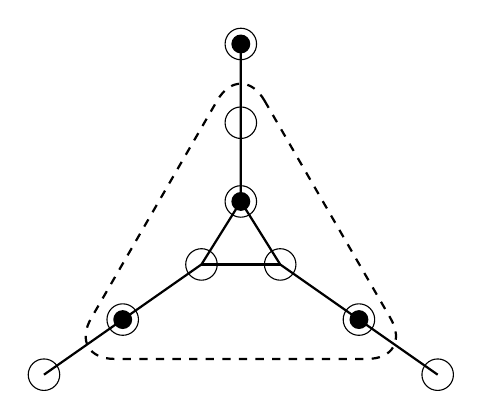
\begin{tikzpicture}
        \def\xb{5}
        \def\yb{0}
        %G_1
        \draw (\xb,\yb+2) circle (0.2cm);         %v9
        \draw (\xb,\yb) circle (0.2cm);           %v1
        \draw (\xb+0.5,\yb-0.8) circle (0.2cm);   %v4
        \draw (\xb-0.5,\yb-0.8) circle (0.2cm);   %v3
        \draw (\xb,\yb+1) circle (0.2cm);         %v2
        \draw (\xb-1.5,\yb-1.5) circle (0.2cm);   %v5
        \draw (\xb+1.5,\yb-1.5) circle (0.2cm);   %v6
        \draw (\xb-2.5,\yb-2.2) circle (0.2cm);     %v7
        \draw (\xb+2.5,\yb-2.2) circle (0.2cm);     %v8

        \path[fill] (\xb,\yb+2) circle (\ver);         %v0
        \path[fill] (\xb,\yb) circle (\ver);           %v1
        \path[fill] (\xb-1.5,\yb-1.5) circle (\ver);   %v5
        \path[fill] (\xb+1.5,\yb-1.5) circle (\ver);   %v6
        %labels
        \draw[thick] (\xb,\yb+2)--(\xb,\yb+1)--(\xb,\yb)--(\xb-0.5,\yb-0.8)--(\xb-1.5,\yb-1.5)--(\xb-2.5,\yb-2.2);
        \draw[thick] (\xb,\yb)--(\xb+0.5,\yb-0.8)--(\xb+1.5,\yb-1.5)--(\xb+2.5,\yb-2.2);
        \draw[thick] (\xb-0.5,\yb-0.8)--(\xb+0.5,\yb-0.8);
        \path[draw, thick, dashed, rounded corners=6mm] (\xb,\yb+1.8)--(\xb+2.2,\yb-2)--(\xb-2.2,\yb-2)--cycle;
      \end{tikzpicture}
    \end{scaletikzpicturetowidth}
    \caption{$OR$ gadget}
    \label{fig:or_gadget_sliding_token}
  \end{subfigure}
  \caption{Sliding Tokens vertex gadgets.}
  \label{fig:and_or_gadgets_sliding_token}
\end{figure}
%%%%%%%%%%%%%%%%%%%%%%%%%%%%%%%%%%%%%%%%%%%%%%%% ENDING OF A FIGURE %%%%%%%%%%%%%%%%%%%%%%%%%%%%%%%%%%%%%%%%%%%%%%%%

\subsubsection{AND/OR Graphs}\label{subsubsection:and_or}
We showed how to construct $AND$ and $OR$ vertices. We now show how to connect the vertices into an arbitrary planar constraint graph.
First, the edges that cross the dotted-line gadget borders are called “port” edges. A token on an outer port-edge vertex represents an
inward-directed NCL edge, and vice-versa. Second, observe that no port token may ever leave its port edge. Choosing a particular port
edge $E$, if we inductively assume that this condition holds for all other port edges, then there is never a legal move outside $E$ for
its token – another port token would have to leave its own edge first.
Given an $AND/OR$ graph $G$ and two legal configurations $C_1, C_2$ for $G$, we construct a corresponding sliding-token graph by joining together
$AND$ and $OR$ vertex gadgets at their shared port edges, placing the port tokens appropriately.


\begin{theorem}Sliding Token problem is $\PSPACE$-complete. \end{theorem}\label{theorem:ncl_sliding_token}
\begin{proof}
  First, we show that SLIDING TOKEN problem is in $\PSPACE$.
  The SLIDING TOKEN problem is in $\PSPACE$ since the state of the input graph can be described in a linear number of bits, specifying the
  position of each token and the list of possible moves from any state can be computed in polynomial time. Thus we can nondeterministically
  traverse the state space, at each step nondeterministically choosing a move to make , and maintaining the current state but not the previously
  visited states showing that SLIDING TOKEN is in $\NPSPACE$. By Savitch's celebrated theorem, we have that $\NPSPACE = \PSPACE$
  \cite{savitch_relationships_1970}, implying that SLIDING TOKEN is in $\PSPACE$.

  The SLIDING TOKEN problem is $\PSPACE$-hard by a reduction from planar Nondeterministic Constraint Logic using the reduction structure
  provided above. The NCL instance is solvable if and only if the corresponding SLIDING TOKEN is solvable.
\end{proof}

\begin{example}{C2E to SLIDING TOKEN problem reduction. \\}
\textbf{Input instance : C2E for restricted NCL.} \hfill

\begin{figure}[H]
  \centering
  \begin{subfigure}[b]{0.4\textwidth}
    \begin{scaletikzpicturetowidth}{\textwidth}
      \begin{tikzpicture}[scale=0.8]
        \def\ver{0.15} %size of a vertex
        % v1
        \def\xa{0}
        \def\ya{0}
        % arrows
        \draw[middlearrow={<}, red] (\xa-2,\ya+1.5)-- (\xa+2,\ya+1.5);        % v2 - v3
        \draw[middlearrow={<}, red] (\xa+2,\ya+1.5) -- (\xa,\ya);             % v3 - v1
        \draw[middlearrow={<}, red] (\xa,\ya) -- (\xa-2,\ya+1.5);             % v1 - v2
        \draw[middlearrow={<}, blue] (\xa-2,\ya+1.5) -- (\xa-2,\ya-3.5);      % v2 - v4
        \draw[middlearrow={<}, blue] (\xa,\ya) -- (\xa,\ya-2);                % v1 - v6
        \draw[middlearrow={<}, blue] (\xa+2,\ya+1.5) -- (\xa+2,\ya-3.5);      % v3 - v5
        \draw[middlearrow={>}, blue] (\xa-2,\ya-3.5) -- (\xa+2,\ya-3.5);      % v4 - v5
        \draw[middlearrow={<}, blue] (\xa-2,\ya-3.5) -- (\xa,\ya-2);          % v4 - v6
        \draw[middlearrow={<}, blue] (\xa,\ya-2) -- (\xa+2,\ya-3.5);          % v6 - v5
        % edges
        \draw[ultra thick, -, red] (\xa-2,\ya+1.5) -- (\xa+2,\ya+1.5);       % v2 - v3
        \draw[ultra thick, -, red] (\xa+2,\ya+1.5) -- (\xa,\ya);             % v3 - v1
        \draw[ultra thick, -, red] (\xa,\ya) -- (\xa-2,\ya+1.5);             % v1 - v2
        \draw[ultra thick, -, blue] (\xa-2,\ya+1.5) -- (\xa-2,\ya-3.5);      % v2 - v4
        \draw[ultra thick, -, blue] (\xa,\ya) -- (\xa,\ya-2);                % v1 - v6
        \draw[ultra thick, -, blue] (\xa+2,\ya+1.5) -- (\xa+2,\ya-3.5);      % v3 - v5
        \draw[ultra thick, -, blue] (\xa-2,\ya-3.5) -- (\xa+2,\ya-3.5);      % v4 - v5
        \draw[ultra thick, -, blue] (\xa-2,\ya-3.5) -- (\xa,\ya-2);          % v4 - v6
        \draw[ultra thick, -, blue] (\xa,\ya-2) -- (\xa+2,\ya-3.5);          % v6 - v5

        \node (a) at (\xa+0.6,\ya-1) {\textbf{E}};

        %graph G : Nodes fill
        \path[fill] (\xa,\ya) circle (\ver);           %v1
        \path[fill] (\xa-2,\ya+1.5) circle (\ver);     %v2
        \path[fill] (\xa+2,\ya+1.5) circle (\ver);     %v3
        \path[fill] (\xa-2,\ya-3.5) circle (\ver);     %v4
        \path[fill] (\xa+2,\ya-3.5) circle (\ver);     %v5
        \path[fill] (\xa,\ya-2) circle (\ver);         %v6
      \end{tikzpicture}
    \end{scaletikzpicturetowidth}
    \caption{$C_0$}
    \label{fig:input_instance}
  \end{subfigure}
  \begin{subfigure}[b]{0.4\textwidth}
    \begin{scaletikzpicturetowidth}{\textwidth}
      \begin{tikzpicture}[scale=0.8]
        \def\ver{0.15} %size of a vertex
        % v1
        \def\xa{0}
        \def\ya{0}
        % Highlight change
        \draw[fill=yellow, opacity=.7, ultra thick, dotted, rotate around={90:(\xa,\ya+1.5)},yellow] (\xa,\ya+1.5) ellipse (10pt and 65pt);
        % f_1 arrows
        \draw[middlearrow={>}, red] (\xa-2,\ya+1.5)-- (\xa+2,\ya+1.5);        % v2 - v3
        \draw[middlearrow={<}, red] (\xa+2,\ya+1.5) -- (\xa,\ya);             % v3 - v1
        \draw[middlearrow={<}, red] (\xa,\ya) -- (\xa-2,\ya+1.5);             % v1 - v2
        \draw[middlearrow={<}, blue] (\xa-2,\ya+1.5) -- (\xa-2,\ya-3.5);      % v2 - v4
        \draw[middlearrow={<}, blue] (\xa,\ya) -- (\xa,\ya-2);                % v1 - v6
        \draw[middlearrow={<}, blue] (\xa+2,\ya+1.5) -- (\xa+2,\ya-3.5);      % v3 - v5
        \draw[middlearrow={>}, blue] (\xa-2,\ya-3.5) -- (\xa+2,\ya-3.5);      % v4 - v5
        \draw[middlearrow={<}, blue] (\xa-2,\ya-3.5) -- (\xa,\ya-2);          % v4 - v6
        \draw[middlearrow={<}, blue] (\xa,\ya-2) -- (\xa+2,\ya-3.5);          % v6 - v5

        \draw[ultra thick, -, red] (\xa-2,\ya+1.5) -- (\xa+2,\ya+1.5);       % v2 - v3
        \draw[ultra thick, -, red] (\xa+2,\ya+1.5) -- (\xa,\ya);             % v3 - v1
        \draw[ultra thick, -, red] (\xa,\ya) -- (\xa-2,\ya+1.5);             % v1 - v2
        \draw[ultra thick, -, blue] (\xa-2,\ya+1.5) -- (\xa-2,\ya-3.5);      % v2 - v4
        \draw[ultra thick, -, blue] (\xa,\ya) -- (\xa,\ya-2);                % v1 - v6
        \draw[ultra thick, -, blue] (\xa+2,\ya+1.5) -- (\xa+2,\ya-3.5);      % v3 - v5
        \draw[ultra thick, -, blue] (\xa-2,\ya-3.5) -- (\xa+2,\ya-3.5);      % v4 - v5
        \draw[ultra thick, -, blue] (\xa-2,\ya-3.5) -- (\xa,\ya-2);          % v4 - v6
        \draw[ultra thick, -, blue] (\xa,\ya-2) -- (\xa+2,\ya-3.5);          % v6 - v5

        \node (a) at (\xa+0.6,\ya-1) {\textbf{E}};

        %graph G : Nodes fill
        \path[fill] (\xa,\ya) circle (\ver);           %v1
        \path[fill] (\xa-2,\ya+1.5) circle (\ver);   %v2
        \path[fill] (\xa+2,\ya+1.5) circle (\ver);   %v3
        \path[fill] (\xa-2,\ya-3.5) circle (\ver);   %v4
        \path[fill] (\xa+2,\ya-3.5) circle (\ver);   %v5
        \path[fill] (\xa,\ya-2) circle (\ver);         %v6
      \end{tikzpicture}
    \end{scaletikzpicturetowidth}
    \caption{$C_1$}
    \label{fig:input_instance_1}
  \end{subfigure}
  \begin{subfigure}[b]{0.4\textwidth}
    \begin{scaletikzpicturetowidth}{\textwidth}
      \begin{tikzpicture}[scale=0.8]
        \def\ver{0.15} %size of a vertex
        % v1
        \def\xa{0}
        \def\ya{0}
        % Highlight change
        \draw[fill=yellow, opacity=.7, ultra thick, dotted, rotate around={305:(\xa+1,\ya+0.75)},yellow] (\xa+1,\ya+0.75) ellipse (10pt and 45pt);
        % f_1 arrows
        \draw[middlearrow={>}, red] (\xa-2,\ya+1.5)-- (\xa+2,\ya+1.5);        % v2 - v3
        \draw[middlearrow={>}, red] (\xa+2,\ya+1.5) -- (\xa,\ya);             % v3 - v1
        \draw[middlearrow={<}, red] (\xa,\ya) -- (\xa-2,\ya+1.5);             % v1 - v2
        \draw[middlearrow={<}, blue] (\xa-2,\ya+1.5) -- (\xa-2,\ya-3.5);      % v2 - v4
        \draw[middlearrow={<}, blue] (\xa,\ya) -- (\xa,\ya-2);                % v1 - v6
        \draw[middlearrow={<}, blue] (\xa+2,\ya+1.5) -- (\xa+2,\ya-3.5);      % v3 - v5
        \draw[middlearrow={>}, blue] (\xa-2,\ya-3.5) -- (\xa+2,\ya-3.5);      % v4 - v5
        \draw[middlearrow={<}, blue] (\xa-2,\ya-3.5) -- (\xa,\ya-2);          % v4 - v6
        \draw[middlearrow={<}, blue] (\xa,\ya-2) -- (\xa+2,\ya-3.5);          % v6 - v5

        \draw[ultra thick, -, red] (\xa-2,\ya+1.5) -- (\xa+2,\ya+1.5);       % v2 - v3
        \draw[ultra thick, -, red] (\xa+2,\ya+1.5) -- (\xa,\ya);             % v3 - v1
        \draw[ultra thick, -, red] (\xa,\ya) -- (\xa-2,\ya+1.5);             % v1 - v2
        \draw[ultra thick, -, blue] (\xa-2,\ya+1.5) -- (\xa-2,\ya-3.5);      % v2 - v4
        \draw[ultra thick, -, blue] (\xa,\ya) -- (\xa,\ya-2);                % v1 - v6
        \draw[ultra thick, -, blue] (\xa+2,\ya+1.5) -- (\xa+2,\ya-3.5);      % v3 - v5
        \draw[ultra thick, -, blue] (\xa-2,\ya-3.5) -- (\xa+2,\ya-3.5);      % v4 - v5
        \draw[ultra thick, -, blue] (\xa-2,\ya-3.5) -- (\xa,\ya-2);          % v4 - v6
        \draw[ultra thick, -, blue] (\xa,\ya-2) -- (\xa+2,\ya-3.5);          % v6 - v5

        \node (a) at (\xa+0.6,\ya-1) {\textbf{E}};

        %graph G : Nodes fill
        \path[fill] (\xa,\ya) circle (\ver);           %v1
        \path[fill] (\xa-2,\ya+1.5) circle (\ver);   %v2
        \path[fill] (\xa+2,\ya+1.5) circle (\ver);   %v3
        \path[fill] (\xa-2,\ya-3.5) circle (\ver);   %v4
        \path[fill] (\xa+2,\ya-3.5) circle (\ver);   %v5
        \path[fill] (\xa,\ya-2) circle (\ver);         %v6
      \end{tikzpicture}
    \end{scaletikzpicturetowidth}
    \caption{$C_2$}
    \label{fig:input_instance_2}
  \end{subfigure}
  \begin{subfigure}[b]{0.4\textwidth}
    \begin{scaletikzpicturetowidth}{\textwidth}
      \begin{tikzpicture}[scale=0.8]
        \def\ver{0.15} %size of a vertex
        % v1
        \def\xa{0}
        \def\ya{0}
        % Highlight change
        \draw[fill=yellow, opacity=.7, ultra thick, dotted, rotate around={180:(\xa,\ya-1)},yellow] (\xa,\ya-1) ellipse (10pt and 45pt);
        % f_1 arrows
        \draw[middlearrow={>}, red] (\xa-2,\ya+1.5)-- (\xa+2,\ya+1.5);        % v2 - v3
        \draw[middlearrow={>}, red] (\xa+2,\ya+1.5) -- (\xa,\ya);             % v3 - v1
        \draw[middlearrow={<}, red] (\xa,\ya) -- (\xa-2,\ya+1.5);             % v1 - v2
        \draw[middlearrow={<}, blue] (\xa-2,\ya+1.5) -- (\xa-2,\ya-3.5);      % v2 - v4
        \draw[middlearrow={>}, blue] (\xa,\ya) -- (\xa,\ya-2);                % v1 - v6
        \draw[middlearrow={<}, blue] (\xa+2,\ya+1.5) -- (\xa+2,\ya-3.5);      % v3 - v5
        \draw[middlearrow={>}, blue] (\xa-2,\ya-3.5) -- (\xa+2,\ya-3.5);      % v4 - v5
        \draw[middlearrow={<}, blue] (\xa-2,\ya-3.5) -- (\xa,\ya-2);          % v4 - v6
        \draw[middlearrow={<}, blue] (\xa,\ya-2) -- (\xa+2,\ya-3.5);          % v6 - v5

        \draw[ultra thick, -, red] (\xa-2,\ya+1.5) -- (\xa+2,\ya+1.5);       % v2 - v3
        \draw[ultra thick, -, red] (\xa+2,\ya+1.5) -- (\xa,\ya);             % v3 - v1
        \draw[ultra thick, -, red] (\xa,\ya) -- (\xa-2,\ya+1.5);             % v1 - v2
        \draw[ultra thick, -, blue] (\xa-2,\ya+1.5) -- (\xa-2,\ya-3.5);      % v2 - v4
        \draw[ultra thick, -, blue] (\xa,\ya) -- (\xa,\ya-2);                % v1 - v6
        \draw[ultra thick, -, blue] (\xa+2,\ya+1.5) -- (\xa+2,\ya-3.5);      % v3 - v5
        \draw[ultra thick, -, blue] (\xa-2,\ya-3.5) -- (\xa+2,\ya-3.5);      % v4 - v5
        \draw[ultra thick, -, blue] (\xa-2,\ya-3.5) -- (\xa,\ya-2);          % v4 - v6
        \draw[ultra thick, -, blue] (\xa,\ya-2) -- (\xa+2,\ya-3.5);          % v6 - v5

        \node (a) at (\xa+0.6,\ya-1) {\textbf{E}};            % Label reject

        %graph G : Nodes fill
        \path[fill] (\xa,\ya) circle (\ver);           %v1
        \path[fill] (\xa-2,\ya+1.5) circle (\ver);   %v2
        \path[fill] (\xa+2,\ya+1.5) circle (\ver);   %v3
        \path[fill] (\xa-2,\ya-3.5) circle (\ver);   %v4
        \path[fill] (\xa+2,\ya-3.5) circle (\ver);   %v5
        \path[fill] (\xa,\ya-2) circle (\ver);         %v6
      \end{tikzpicture}
    \end{scaletikzpicturetowidth}
    \caption{$C_3$}
    \label{fig:input_instance_3}
  \end{subfigure}
  \caption{Reconfiguration sequence which transforms $C_0$ which is the initial configuration into $C_3 = $ which is the target configuration.}
  \label{fig:input_instance_config_to_edge}
\end{figure}

%%%%%%%%%%%%%%%%%%%%%%%%%%%%%%%%%%%%%%%%%%% Output instance %%%%%%%%%%%%%%%%%%%%%%%%%%%%%%%%
%------------------------------------------- out 1 & 2 ---------------------------------------------
\textbf{Output instance : SLIDING TOKEN instance.} \hfill

\begin{figure}[H]
  \raggedright
  \begin{subfigure}[b]{0.6\textwidth}
    \begin{scaletikzpicturetowidth}{\textwidth}
      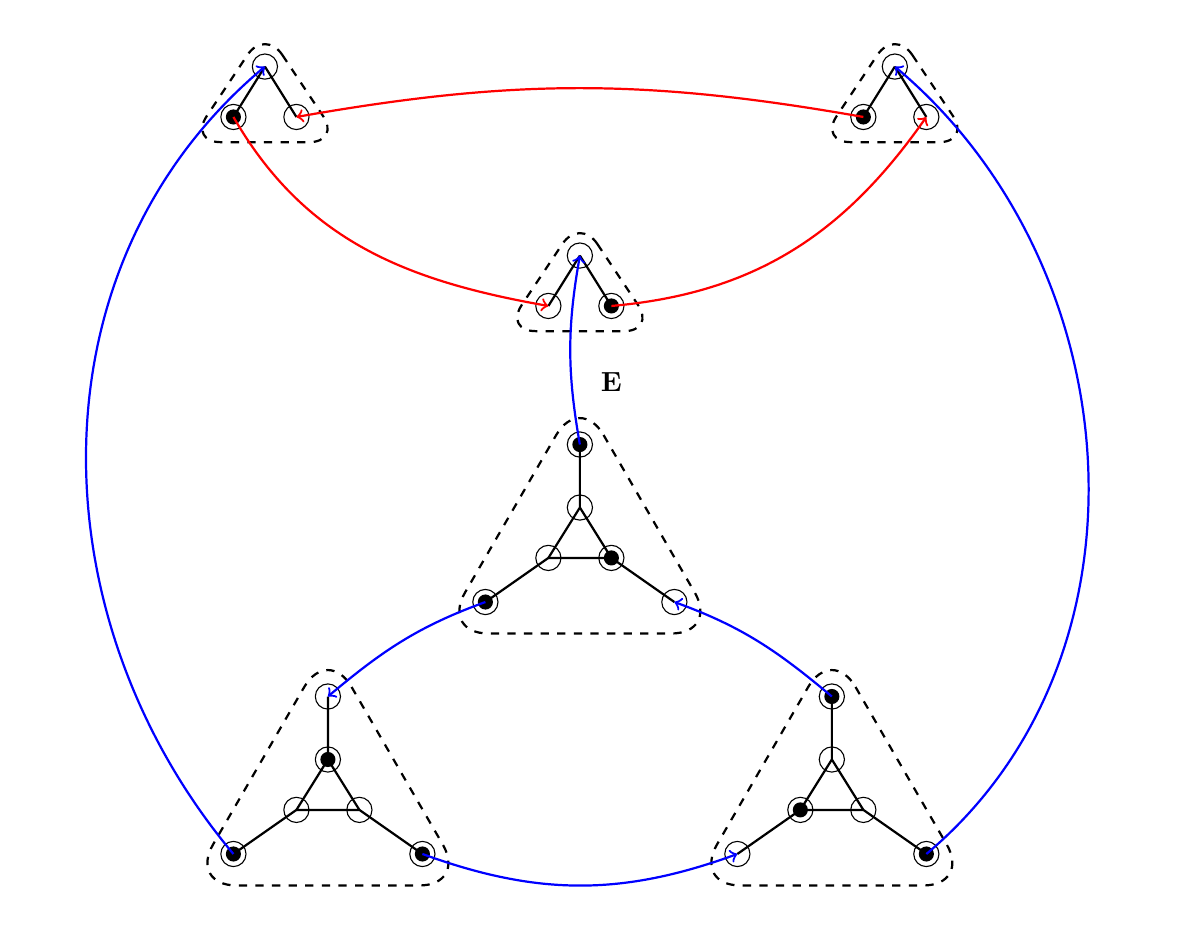
\begin{tikzpicture}[scale=0.8]
        %%%%%%%%%%%% AND 1 %%%%%%%%%%%%
        \def\ver{0.12} %size of a vertex
        \def\xa{-1}
        \def\ya{0}
        % Highlight change
        %graph G
        \draw (\xa,\ya) circle (0.2cm);          %v1 no fill
        \draw (\xa+0.5,\ya-0.8) circle (0.2cm);  %v4 no fill
        \draw (\xa-0.5,\ya-0.8) circle (0.2cm);  %v3 no fill
        % Tokens
        \path[fill] (\xa-0.5,\ya-0.8) circle (\ver);   %v3
        %labels
        \draw[thick] (\xa,\ya)--(\xa-0.5,\ya-0.8);
        \draw[thick] (\xa,\ya)--(\xa+0.5,\ya-0.8);
        \path[draw, thick, dashed, rounded corners=4mm] (\xa,\ya+0.6)--(\xa+1.2,\ya-1.2)--(\xa-1.2,\ya-1.2)--cycle;
        %%%%%%%%%%%% AND 2 %%%%%%%%%%%%
        \def\ver{0.12} %size of a vertex
        \def\xb{4}
        \def\yb{-3}
        %graph G
        \draw (\xb,\yb) circle (0.2cm);          %v1 no fill
        \draw (\xb+0.5,\yb-0.8) circle (0.2cm);  %v4 no fill
        \draw (\xb-0.5,\yb-0.8) circle (0.2cm);  %v3 no fill
        % Tokens
        \path[fill] (\xb+0.5,\yb-0.8) circle (\ver);   %v3
        %labels
        \draw[thick] (\xb,\yb)--(\xb-0.5,\yb-0.8);
        \draw[thick] (\xb,\yb)--(\xb+0.5,\yb-0.8);
        \path[draw, thick, dashed, rounded corners=4mm] (\xb,\yb+0.6)--(\xb+1.2,\yb-1.2)--(\xb-1.2,\yb-1.2)--cycle;
        %%%%%%%%%%%% AND 3 %%%%%%%%%%%%
        \def\ver{0.12} %size of a vertex
        \def\xc{9}
        \def\yc{0}
        %graph G
        \draw (\xc,\yc) circle (0.2cm);          %v1 no fill
        \draw (\xc+0.5,\yc-0.8) circle (0.2cm);  %v4 no fill
        \draw (\xc-0.5,\yc-0.8) circle (0.2cm);  %v3 no fill
        % Tokens
        \path[fill] (\xc-0.5,\yc-0.8) circle (\ver);   %v3
        %labels
        \draw[thick] (\xc,\yc)--(\xc-0.5,\yc-0.8);
        \draw[thick] (\xc,\yc)--(\xc+0.5,\yc-0.8);
        \path[draw, thick, dashed, rounded corners=4mm] (\xc,\yc+0.6)--(\xc+1.2,\yc-1.2)--(\xc-1.2,\yc-1.2)--cycle;
        %%%%%%%%%%%% OR 1 %%%%%%%%%%%%
        \def\ver{0.12} %size of a vertex
        \def\xd{0}
        \def\yd{-11}
        %G_1
        \draw (\xd,\yd) circle (0.2cm);           %v1
        \draw (\xd+0.5,\yd-0.8) circle (0.2cm);   %v4
        \draw (\xd-0.5,\yd-0.8) circle (0.2cm);   %v3
        \draw (\xd,\yd+1) circle (0.2cm);         %v2
        \draw (\xd-1.5,\yd-1.5) circle (0.2cm);   %v5
        \draw (\xd+1.5,\yd-1.5) circle (0.2cm);   %v6
        \path[fill] (\xd,\yd) circle (\ver);           %v1
        \path[fill] (\xd-1.5,\yd-1.5) circle (\ver);   %v5
        \path[fill] (\xd+1.5,\yd-1.5) circle (\ver);   %v6
        %labels
        \draw[thick] (\xd,\yd+1)--(\xd, \yd)--(\xd-0.5,\yd-0.8)--(\xd-1.5,\yd-1.5);
        \draw[thick] (\xd-0.5,\yd-0.8)--(\xd+0.5,\yd-0.8)--(\xd+1.5,\yd-1.5);
        \draw[thick] (\xd,\yd)-- (\xd+0.5,\yd-0.8);

        \path[draw, thick, dashed, rounded corners=6mm] (\xd,\yd+1.8)--(\xd+2.2,\yd-2)--(\xd-2.2,\yd-2)--cycle;
        %%%%%%%%%%%% OR 2 %%%%%%%%%%%%
        \def\ver{0.12} %size of a vertex
        \def\xe{4}
        \def\ye{-7}
        %G_1
        \draw (\xe,\ye) circle (0.2cm);           %v1
        \draw (\xe+0.5,\ye-0.8) circle (0.2cm);   %v4
        \draw (\xe-0.5,\ye-0.8) circle (0.2cm);   %v3
        \draw (\xe,\ye+1) circle (0.2cm);         %v2
        \draw (\xe-1.5,\ye-1.5) circle (0.2cm);   %v5
        \draw (\xe+1.5,\ye-1.5) circle (0.2cm);   %v6

        \path[fill] (\xe,\ye+1) circle (\ver);         %v2
        \path[fill] (\xe+0.5,\ye-0.8) circle (\ver);   %v4
        \path[fill] (\xe-1.5,\ye-1.5) circle (\ver);   %v5
        %labels
        \draw[thick] (\xe,\ye+1)--(\xe, \ye)--(\xe-0.5,\ye-0.8)--(\xe-1.5,\ye-1.5);
        \draw[thick] (\xe-0.5,\ye-0.8)--(\xe+0.5,\ye-0.8)--(\xe+1.5,\ye-1.5);
        \draw[thick] (\xe,\ye)-- (\xe+0.5,\ye-0.8);
        \path[draw, thick, dashed, rounded corners=6mm] (\xe,\ye+1.8)--(\xe+2.2,\ye-2)--(\xe-2.2,\ye-2)--cycle;
        %%%%%%%%%%%% OR 3 %%%%%%%%%%%%
        \def\ver{0.12} %size of a vertex
        \def\xf{8}
        \def\yf{-11}
        %G_1
        \draw (\xf,\yf) circle (0.2cm);           %v1
        \draw (\xf+0.5,\yf-0.8) circle (0.2cm);   %v4
        \draw (\xf-0.5,\yf-0.8) circle (0.2cm);   %v3
        \draw (\xf,\yf+1) circle (0.2cm);         %v2
        \draw (\xf-1.5,\yf-1.5) circle (0.2cm);   %v5
        \draw (\xf+1.5,\yf-1.5) circle (0.2cm);   %v6

        \path[fill] (\xf,\yf+1) circle (\ver);         %v2
        \path[fill] (\xf-0.5,\yf-0.8) circle (\ver);   %v3
        \path[fill] (\xf+1.5,\yf-1.5) circle (\ver);   %v6
        %labels
        \draw[thick] (\xf,\yf+1)--(\xf, \yf)--(\xf-0.5,\yf-0.8)--(\xf-1.5,\yf-1.5);
        \draw[thick] (\xf-0.5,\yf-0.8)--(\xf+0.5,\yf-0.8)--(\xf+1.5,\yf-1.5);
        \draw[thick] (\xf,\yf)-- (\xf+0.5,\yf-0.8);
        \path[draw, thick, dashed, rounded corners=6mm] (\xf,\yf+1.8)--(\xf+2.2,\yf-2)--(\xf-2.2,\yf-2)--cycle;
        %%%%%%%%%%% EDGES %%%%%%%%%
        \node (a) at (4.5,-5) {\textbf{E}};            % Label reject
        \draw [-, red, thick, arrows={->[scale=3,red]}] (\xc-0.5,\yc-0.8) to [out=170,in=10] (\xa+0.5,\ya-0.8);            % AND 3  -- AND 1
        \draw [-, red, thick, arrows={->[scale=3,red]}] (\xa-0.5,\ya-0.8)  to [out=300,in=170] (\xb-0.5,\yb-0.8);          % AND 1  -- AND 2
        \draw [-, red, thick, arrows={->[scale=3,red]}] (\xb+0.5,\yb-0.8) to [out=5,in=235] (\xc+0.5,\yc-0.8);             % AND 2  -- AND 3
        \draw [-, blue, thick, arrows={->[scale=3,blue]}] (\xd-1.5,\yd-1.5) to [out=130,in=220] (\xa,\ya);                 % OR 1  -- AND 1
        \draw [-, blue, thick, arrows={->[scale=3,blue]}] (\xd+1.5,\yd-1.5) to [out=340,in=200] (\xf-1.5,\yf-1.5);         % OR 1  -- OR 3
        \draw [-, blue, thick, arrows={->[scale=3,blue]}] (\xf,\yf+1)  to [out=140,in=340] (\xe+1.5,\ye-1.5);              % OR 3  -- OR 2
        \draw [-, blue, thick, arrows={->[scale=3,blue]}] (\xe-1.5,\ye-1.5) to [out=200,in=40] (\xd,\yd+1);                % OR 2  -- OR 1
        \draw [-, blue, thick, arrows={->[scale=3,blue]}] (\xf+1.5,\yf-1.5) to [out=40,in=320] (\xc,\yc);                  % OR 3  -- AND 3
        \draw [-, blue, thick, arrows={->[scale=3,blue]}] (\xe,\ye+1) to [out=100,in=260] (\xb,\yb);                       % OR 2  -- AND 2
      \end{tikzpicture}
    \end{scaletikzpicturetowidth}
  \caption{$S_0$.}
  \label{fig:output_instance_final}
  \end{subfigure}
  \vspace{3em}
  \begin{subfigure}[b]{0.6\textwidth}
    \begin{scaletikzpicturetowidth}{\textwidth}
      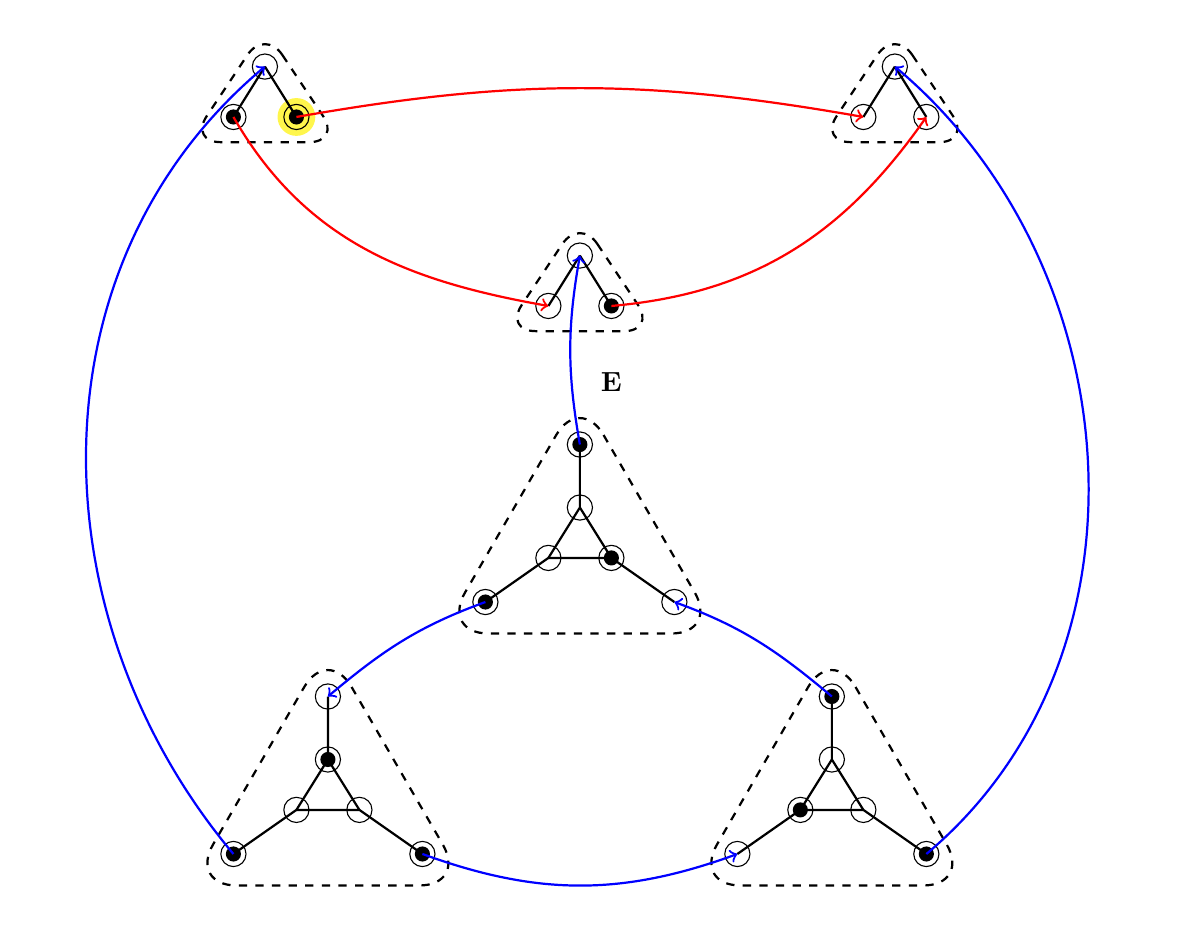
\begin{tikzpicture}[scale=0.8]
        %%%%%%%%%%%% AND 1 %%%%%%%%%%%%
        \def\ver{0.12} %size of a vertex
        \def\xa{-1}
        \def\ya{0}
        % Highlight change
        \draw[fill=yellow, opacity=.7, draw=none] (\xa+0.5,\ya-0.8) circle (0.3cm);
        %\draw[fill=yellow, opacity=.7, draw=none] (\xa-0.5,\ya-0.8) circle (0.3cm);
        %graph G
        \draw (\xa,\ya) circle (0.2cm);          %v1 no fill
        \draw (\xa+0.5,\ya-0.8) circle (0.2cm);  %v4 no fill
        \draw (\xa-0.5,\ya-0.8) circle (0.2cm);  %v3 no fill
        % Tokens
        \path[fill] (\xa-0.5,\ya-0.8) circle (\ver);   %v3
        \path[fill] (\xa+0.5,\ya-0.8) circle (\ver);   %v4
        %labels
        \draw[thick] (\xa,\ya)--(\xa-0.5,\ya-0.8);
        \draw[thick] (\xa,\ya)--(\xa+0.5,\ya-0.8);
        \path[draw, thick, dashed, rounded corners=4mm] (\xa,\ya+0.6)--(\xa+1.2,\ya-1.2)--(\xa-1.2,\ya-1.2)--cycle;
        %%%%%%%%%%%% AND 2 %%%%%%%%%%%%
        \def\ver{0.12} %size of a vertex
        \def\xb{4}
        \def\yb{-3}
        %graph G
        \draw (\xb,\yb) circle (0.2cm);          %v1 no fill
        \draw (\xb+0.5,\yb-0.8) circle (0.2cm);  %v4 no fill
        \draw (\xb-0.5,\yb-0.8) circle (0.2cm);  %v3 no fill
        % Tokens
        \path[fill] (\xb+0.5,\yb-0.8) circle (\ver);   %v3
        %labels
        \draw[thick] (\xb,\yb)--(\xb-0.5,\yb-0.8);
        \draw[thick] (\xb,\yb)--(\xb+0.5,\yb-0.8);
        \path[draw, thick, dashed, rounded corners=4mm] (\xb,\yb+0.6)--(\xb+1.2,\yb-1.2)--(\xb-1.2,\yb-1.2)--cycle;
        %%%%%%%%%%%% AND 3 %%%%%%%%%%%%
        \def\ver{0.12} %size of a vertex
        \def\xc{9}
        \def\yc{0}
        %graph G
        \draw (\xc,\yc) circle (0.2cm);          %v1 no fill
        \draw (\xc+0.5,\yc-0.8) circle (0.2cm);  %v4 no fill
        \draw (\xc-0.5,\yc-0.8) circle (0.2cm);  %v3 no fill
        %labels
        \draw[thick] (\xc,\yc)--(\xc-0.5,\yc-0.8);
        \draw[thick] (\xc,\yc)--(\xc+0.5,\yc-0.8);
        \path[draw, thick, dashed, rounded corners=4mm] (\xc,\yc+0.6)--(\xc+1.2,\yc-1.2)--(\xc-1.2,\yc-1.2)--cycle;
        %%%%%%%%%%%% OR 1 %%%%%%%%%%%%
        \def\ver{0.12} %size of a vertex
        \def\xd{0}
        \def\yd{-11}
        %G_1
        \draw (\xd,\yd) circle (0.2cm);           %v1
        \draw (\xd+0.5,\yd-0.8) circle (0.2cm);   %v4
        \draw (\xd-0.5,\yd-0.8) circle (0.2cm);   %v3
        \draw (\xd,\yd+1) circle (0.2cm);         %v2
        \draw (\xd-1.5,\yd-1.5) circle (0.2cm);   %v5
        \draw (\xd+1.5,\yd-1.5) circle (0.2cm);   %v6

        \path[fill] (\xd,\yd) circle (\ver);           %v1
        \path[fill] (\xd-1.5,\yd-1.5) circle (\ver);   %v5
        \path[fill] (\xd+1.5,\yd-1.5) circle (\ver);   %v6
        %labels
        \draw[thick] (\xd,\yd+1)--(\xd, \yd)--(\xd-0.5,\yd-0.8)--(\xd-1.5,\yd-1.5);
        \draw[thick] (\xd-0.5,\yd-0.8)--(\xd+0.5,\yd-0.8)--(\xd+1.5,\yd-1.5);
        \draw[thick] (\xd,\yd)-- (\xd+0.5,\yd-0.8);
        \path[draw, thick, dashed, rounded corners=6mm] (\xd,\yd+1.8)--(\xd+2.2,\yd-2)--(\xd-2.2,\yd-2)--cycle;
        %%%%%%%%%%%% OR 2 %%%%%%%%%%%%
        \def\ver{0.12} %size of a vertex
        \def\xe{4}
        \def\ye{-7}
        %G_1
        \draw (\xe,\ye) circle (0.2cm);           %v1
        \draw (\xe+0.5,\ye-0.8) circle (0.2cm);   %v4
        \draw (\xe-0.5,\ye-0.8) circle (0.2cm);   %v3
        \draw (\xe,\ye+1) circle (0.2cm);         %v2
        \draw (\xe-1.5,\ye-1.5) circle (0.2cm);   %v5
        \draw (\xe+1.5,\ye-1.5) circle (0.2cm);   %v6
        \path[fill] (\xe,\ye+1) circle (\ver);         %v2
        \path[fill] (\xe+0.5,\ye-0.8) circle (\ver);   %v4
        \path[fill] (\xe-1.5,\ye-1.5) circle (\ver);   %v5
        %labels
        \draw[thick] (\xe,\ye+1)--(\xe, \ye)--(\xe-0.5,\ye-0.8)--(\xe-1.5,\ye-1.5);
        \draw[thick] (\xe-0.5,\ye-0.8)--(\xe+0.5,\ye-0.8)--(\xe+1.5,\ye-1.5);
        \draw[thick] (\xe,\ye)-- (\xe+0.5,\ye-0.8);
        \path[draw, thick, dashed, rounded corners=6mm] (\xe,\ye+1.8)--(\xe+2.2,\ye-2)--(\xe-2.2,\ye-2)--cycle;
        %%%%%%%%%%%% OR 3 %%%%%%%%%%%%
        \def\ver{0.12} %size of a vertex
        \def\xf{8}
        \def\yf{-11}
        %G_1
        \draw (\xf,\yf) circle (0.2cm);           %v1
        \draw (\xf+0.5,\yf-0.8) circle (0.2cm);   %v4
        \draw (\xf-0.5,\yf-0.8) circle (0.2cm);   %v3
        \draw (\xf,\yf+1) circle (0.2cm);         %v2
        \draw (\xf-1.5,\yf-1.5) circle (0.2cm);   %v5
        \draw (\xf+1.5,\yf-1.5) circle (0.2cm);   %v6
        %tokens
        \path[fill] (\xf,\yf+1) circle (\ver);         %v2
        \path[fill] (\xf-0.5,\yf-0.8) circle (\ver);   %v3
        \path[fill] (\xf+1.5,\yf-1.5) circle (\ver);   %v6
        %labels
        \draw[thick] (\xf,\yf+1)--(\xf, \yf)--(\xf-0.5,\yf-0.8)--(\xf-1.5,\yf-1.5);
        \draw[thick] (\xf-0.5,\yf-0.8)--(\xf+0.5,\yf-0.8)--(\xf+1.5,\yf-1.5);
        \draw[thick] (\xf,\yf)-- (\xf+0.5,\yf-0.8);
        \path[draw, thick, dashed, rounded corners=6mm] (\xf,\yf+1.8)--(\xf+2.2,\yf-2)--(\xf-2.2,\yf-2)--cycle;
        %%%%%%%%%%% EDGES %%%%%%%%%
        \node (a) at (4.5,-5) {\textbf{E}};            % Label reject
        \draw [-, red, thick, arrows={->[scale=3,red]}]  (\xa+0.5,\ya-0.8) to [out=10,in=170]  (\xc-0.5,\yc-0.8);          % AND 1  -- AND 3
        \draw [-, red, thick, arrows={->[scale=3,red]}] (\xa-0.5,\ya-0.8)  to [out=300,in=170] (\xb-0.5,\yb-0.8);          % AND 1  -- AND 2
        \draw [-, red, thick, arrows={->[scale=3,red]}] (\xb+0.5,\yb-0.8) to [out=5,in=235] (\xc+0.5,\yc-0.8);             % AND 2  -- AND 3
        \draw [-, blue, thick, arrows={->[scale=3,blue]}] (\xd-1.5,\yd-1.5) to [out=130,in=220] (\xa,\ya);                 % OR 1  -- AND 1
        \draw [-, blue, thick, arrows={->[scale=3,blue]}] (\xd+1.5,\yd-1.5) to [out=340,in=200] (\xf-1.5,\yf-1.5);         % OR 1  -- OR 3
        \draw [-, blue, thick, arrows={->[scale=3,blue]}] (\xf,\yf+1)  to [out=140,in=340] (\xe+1.5,\ye-1.5);              % OR 3  -- OR 2
        \draw [-, blue, thick, arrows={->[scale=3,blue]}] (\xe-1.5,\ye-1.5) to [out=200,in=40] (\xd,\yd+1);                % OR 2  -- OR 1
        \draw [-, blue, thick, arrows={->[scale=3,blue]}] (\xf+1.5,\yf-1.5) to [out=40,in=320] (\xc,\yc);                  % OR 3  -- AND 3
        \draw [-, blue, thick, arrows={->[scale=3,blue]}] (\xe,\ye+1) to [out=100,in=260] (\xb,\yb);                       % OR 2  -- AND 2
      \end{tikzpicture}
    \end{scaletikzpicturetowidth}
    \caption{$S_1.$}
    \label{fig:output_instance_final}
  \end{subfigure}
\end{figure}


%------------------------------------------- out 3 & 4 ---------------------------------------------
\begin{figure}[H]\ContinuedFloat
  \raggedright
  \begin{subfigure}[b]{0.6\textwidth}
    \begin{scaletikzpicturetowidth}{\textwidth}
      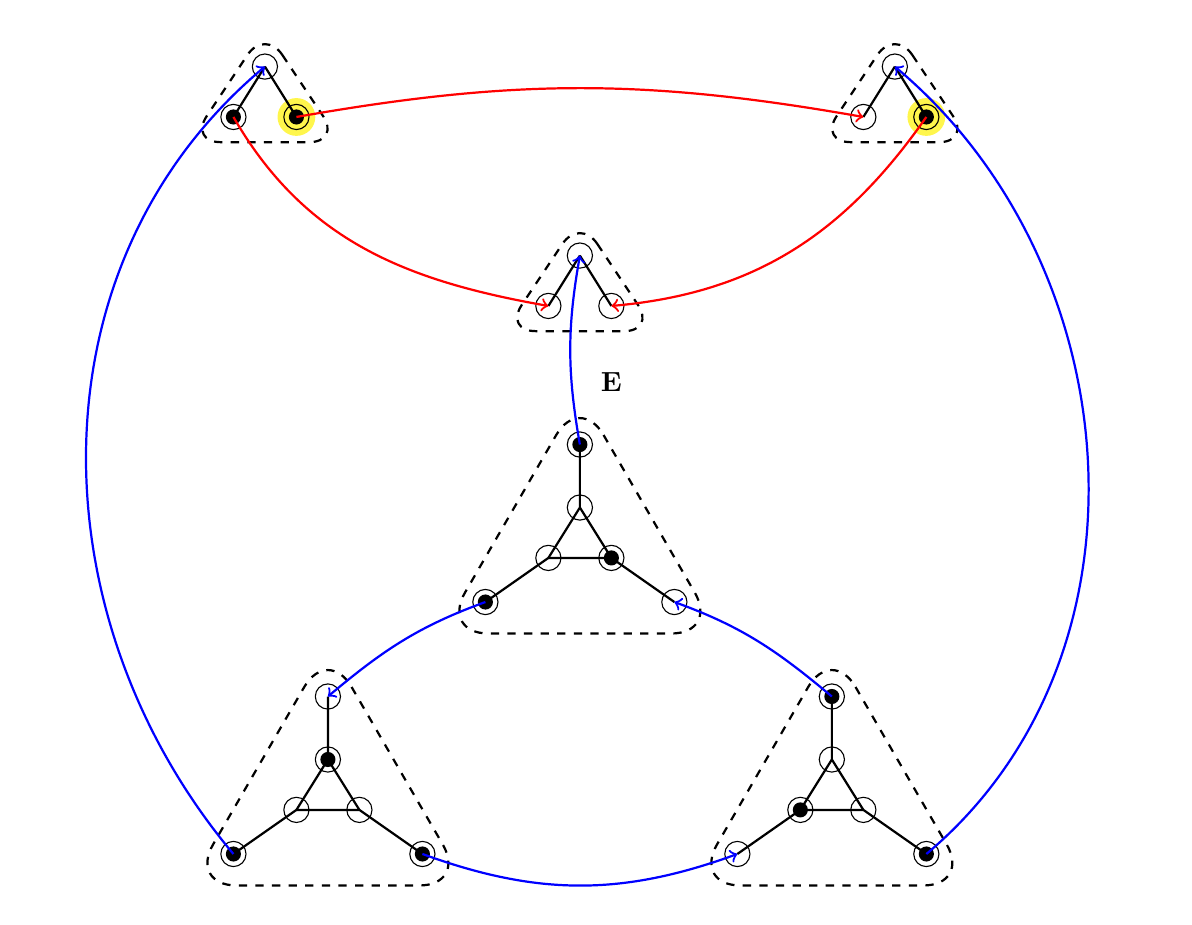
\begin{tikzpicture}[scale=0.8]
        %%%%%%%%%%%% AND 1 %%%%%%%%%%%%
        \def\ver{0.12} %size of a vertex
        \def\xa{-1}
        \def\ya{0}
        % Highlight change
        \draw[fill=yellow, opacity=.7, draw=none] (\xa+0.5,\ya-0.8) circle (0.3cm);
        %\draw[fill=yellow, opacity=.7, draw=none] (\xa-0.5,\ya-0.8) circle (0.3cm);
        %graph G
        \draw (\xa,\ya) circle (0.2cm);          %v1 no fill
        \draw (\xa+0.5,\ya-0.8) circle (0.2cm);  %v4 no fill
        \draw (\xa-0.5,\ya-0.8) circle (0.2cm);  %v3 no fill
        % Tokens
        \path[fill] (\xa-0.5,\ya-0.8) circle (\ver);   %v3
        \path[fill] (\xa+0.5,\ya-0.8) circle (\ver);   %v4
        %labels
        \draw[thick] (\xa,\ya)--(\xa-0.5,\ya-0.8);
        \draw[thick] (\xa,\ya)--(\xa+0.5,\ya-0.8);
        \path[draw, thick, dashed, rounded corners=4mm] (\xa,\ya+0.6)--(\xa+1.2,\ya-1.2)--(\xa-1.2,\ya-1.2)--cycle;
        %%%%%%%%%%%% AND 2 %%%%%%%%%%%%
        \def\ver{0.12} %size of a vertex
        \def\xb{4}
        \def\yb{-3}
        %graph G
        \draw (\xb,\yb) circle (0.2cm);          %v1 no fill
        \draw (\xb+0.5,\yb-0.8) circle (0.2cm);  %v4 no fill
        \draw (\xb-0.5,\yb-0.8) circle (0.2cm);  %v3 no fill
        %labels
        \draw[thick] (\xb,\yb)--(\xb-0.5,\yb-0.8);
        \draw[thick] (\xb,\yb)--(\xb+0.5,\yb-0.8);
        \path[draw, thick, dashed, rounded corners=4mm] (\xb,\yb+0.6)--(\xb+1.2,\yb-1.2)--(\xb-1.2,\yb-1.2)--cycle;
        %%%%%%%%%%%% AND 3 %%%%%%%%%%%%
        \def\ver{0.12} %size of a vertex
        \def\xc{9}
        \def\yc{0}
        % Highlight
        \draw[fill=yellow, opacity=.7, draw=none] (\xc+0.5,\yc-0.8) circle (0.3cm);
        %graph G
        \draw (\xc,\yc) circle (0.2cm);          %v1 no fill
        \draw (\xc+0.5,\yc-0.8) circle (0.2cm);  %v4 no fill
        \draw (\xc-0.5,\yc-0.8) circle (0.2cm);  %v3 no fill
        % Tokens
        \path[fill] (\xc+0.5,\yc-0.8) circle (\ver);   %v4
        %labels
        \draw[thick] (\xc,\yc)--(\xc-0.5,\yc-0.8);
        \draw[thick] (\xc,\yc)--(\xc+0.5,\yc-0.8);
        \path[draw, thick, dashed, rounded corners=4mm] (\xc,\yc+0.6)--(\xc+1.2,\yc-1.2)--(\xc-1.2,\yc-1.2)--cycle;
        %%%%%%%%%%%% OR 1 %%%%%%%%%%%%
        \def\ver{0.12} %size of a vertex
        \def\xd{0}
        \def\yd{-11}
        %G_1
        \draw (\xd,\yd) circle (0.2cm);           %v1
        \draw (\xd+0.5,\yd-0.8) circle (0.2cm);   %v4
        \draw (\xd-0.5,\yd-0.8) circle (0.2cm);   %v3
        \draw (\xd,\yd+1) circle (0.2cm);         %v2
        \draw (\xd-1.5,\yd-1.5) circle (0.2cm);   %v5
        \draw (\xd+1.5,\yd-1.5) circle (0.2cm);   %v6
        % tokens
        \path[fill] (\xd,\yd) circle (\ver);           %v1
        \path[fill] (\xd-1.5,\yd-1.5) circle (\ver);   %v5
        \path[fill] (\xd+1.5,\yd-1.5) circle (\ver);   %v6
        %labels
        \draw[thick] (\xd,\yd+1)--(\xd, \yd)--(\xd-0.5,\yd-0.8)--(\xd-1.5,\yd-1.5);
        \draw[thick] (\xd-0.5,\yd-0.8)--(\xd+0.5,\yd-0.8)--(\xd+1.5,\yd-1.5);
        \draw[thick] (\xd,\yd)-- (\xd+0.5,\yd-0.8);
        %edges
        \path[draw, thick, dashed, rounded corners=6mm] (\xd,\yd+1.8)--(\xd+2.2,\yd-2)--(\xd-2.2,\yd-2)--cycle;
        %%%%%%%%%%%% OR 2 %%%%%%%%%%%%
        \def\ver{0.12} %size of a vertex
        \def\xe{4}
        \def\ye{-7}
        %G_1
        \draw (\xe,\ye) circle (0.2cm);           %v1
        \draw (\xe+0.5,\ye-0.8) circle (0.2cm);   %v4
        \draw (\xe-0.5,\ye-0.8) circle (0.2cm);   %v3
        \draw (\xe,\ye+1) circle (0.2cm);         %v2
        \draw (\xe-1.5,\ye-1.5) circle (0.2cm);   %v5
        \draw (\xe+1.5,\ye-1.5) circle (0.2cm);   %v6
        % token
        \path[fill] (\xe,\ye+1) circle (\ver);         %v2
        \path[fill] (\xe+0.5,\ye-0.8) circle (\ver);   %v4
        \path[fill] (\xe-1.5,\ye-1.5) circle (\ver);   %v5
        %labels
        \draw[thick] (\xe,\ye+1)--(\xe, \ye)--(\xe-0.5,\ye-0.8)--(\xe-1.5,\ye-1.5);
        \draw[thick] (\xe-0.5,\ye-0.8)--(\xe+0.5,\ye-0.8)--(\xe+1.5,\ye-1.5);
        \draw[thick] (\xe,\ye)-- (\xe+0.5,\ye-0.8);

        \path[draw, thick, dashed, rounded corners=6mm] (\xe,\ye+1.8)--(\xe+2.2,\ye-2)--(\xe-2.2,\ye-2)--cycle;

        %%%%%%%%%%%% OR 3 %%%%%%%%%%%%
        \def\ver{0.12} %size of a vertex
        \def\xf{8}
        \def\yf{-11}
        %G_1
        \draw (\xf,\yf) circle (0.2cm);           %v1
        \draw (\xf+0.5,\yf-0.8) circle (0.2cm);   %v4
        \draw (\xf-0.5,\yf-0.8) circle (0.2cm);   %v3
        \draw (\xf,\yf+1) circle (0.2cm);         %v2
        \draw (\xf-1.5,\yf-1.5) circle (0.2cm);   %v5
        \draw (\xf+1.5,\yf-1.5) circle (0.2cm);   %v6

        \path[fill] (\xf,\yf+1) circle (\ver);         %v2
        \path[fill] (\xf-0.5,\yf-0.8) circle (\ver);   %v3
        \path[fill] (\xf+1.5,\yf-1.5) circle (\ver);   %v6
        %labels
        \draw[thick] (\xf,\yf+1)--(\xf, \yf)--(\xf-0.5,\yf-0.8)--(\xf-1.5,\yf-1.5);
        \draw[thick] (\xf-0.5,\yf-0.8)--(\xf+0.5,\yf-0.8)--(\xf+1.5,\yf-1.5);
        \draw[thick] (\xf,\yf)-- (\xf+0.5,\yf-0.8);

        \path[draw, thick, dashed, rounded corners=6mm] (\xf,\yf+1.8)--(\xf+2.2,\yf-2)--(\xf-2.2,\yf-2)--cycle;
        %%%%%%%%%%% EDGES %%%%%%%%%
        \node (a) at (4.5,-5) {\textbf{E}};            % Label reject
        \draw [-, red, thick, arrows={->[scale=3,red]}]  (\xa+0.5,\ya-0.8) to [out=10,in=170]  (\xc-0.5,\yc-0.8);          % AND 1  -- AND 3
        \draw [-, red, thick, arrows={->[scale=3,red]}] (\xa-0.5,\ya-0.8)  to [out=300,in=170] (\xb-0.5,\yb-0.8);          % AND 1  -- AND 2
        \draw [-, red, thick, arrows={->[scale=3,red]}] (\xc+0.5,\yc-0.8) to [out=235,in=5] (\xb+0.5,\yb-0.8) ;            % AND 3  -- AND 2
        \draw [-, blue, thick, arrows={->[scale=3,blue]}] (\xd-1.5,\yd-1.5) to [out=130,in=220] (\xa,\ya);                 % OR 1  -- AND 1
        \draw [-, blue, thick, arrows={->[scale=3,blue]}] (\xd+1.5,\yd-1.5) to [out=340,in=200] (\xf-1.5,\yf-1.5);         % OR 1  -- OR 3
        \draw [-, blue, thick, arrows={->[scale=3,blue]}] (\xf,\yf+1)  to [out=140,in=340] (\xe+1.5,\ye-1.5);              % OR 3  -- OR 2
        \draw [-, blue, thick, arrows={->[scale=3,blue]}] (\xe-1.5,\ye-1.5) to [out=200,in=40] (\xd,\yd+1);                % OR 2  -- OR 1
        \draw [-, blue, thick, arrows={->[scale=3,blue]}] (\xf+1.5,\yf-1.5) to [out=40,in=320] (\xc,\yc);                  % OR 3  -- AND 3
        \draw [-, blue, thick, arrows={->[scale=3,blue]}] (\xe,\ye+1) to [out=100,in=260] (\xb,\yb);                       % OR 2  -- AND 2
      \end{tikzpicture}
    \end{scaletikzpicturetowidth}
    \caption{$S_2.$}
    \label{fig:output_instance_final}
  \end{subfigure}
  \vspace{3em}
  \begin{subfigure}[b]{0.6\textwidth}
    \begin{scaletikzpicturetowidth}{\textwidth}
      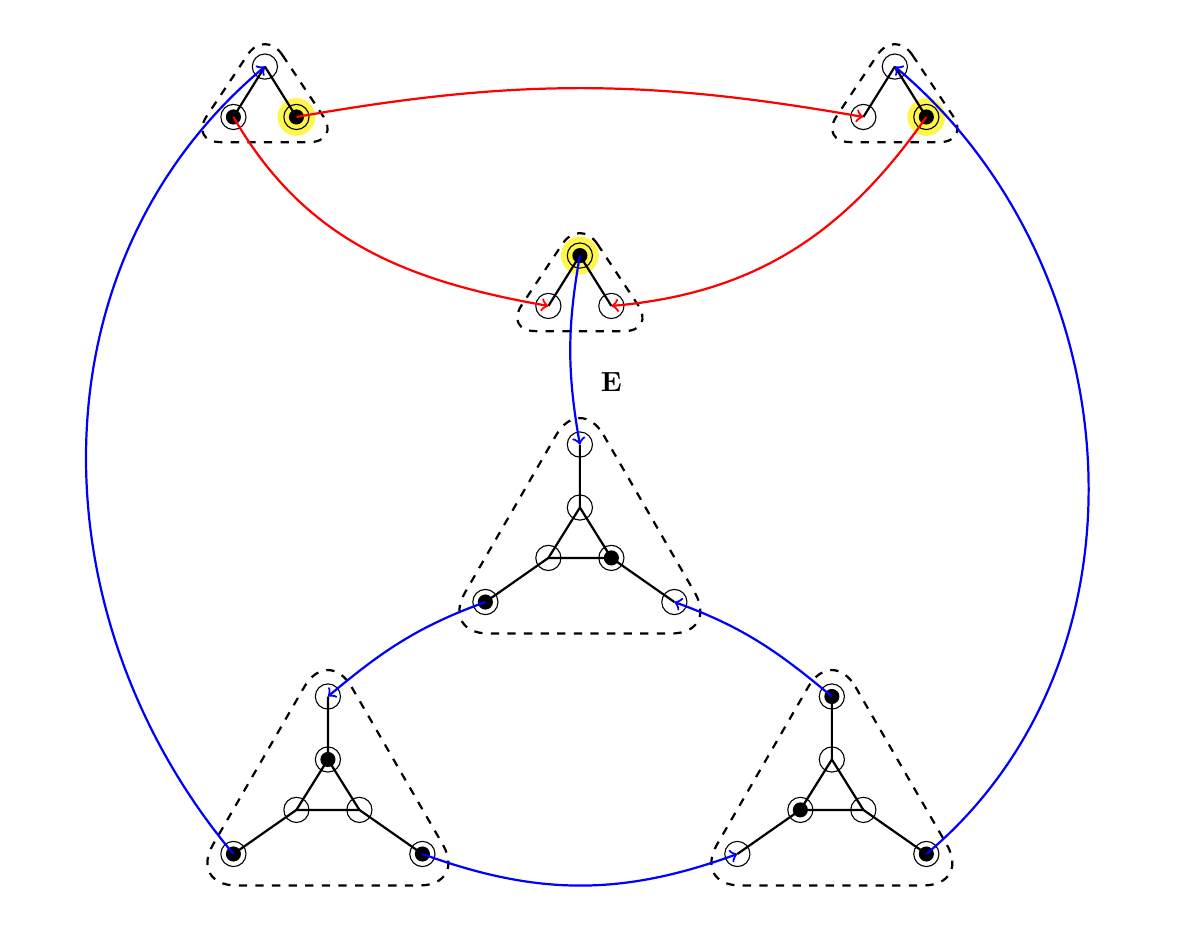
\begin{tikzpicture}[scale=0.8]
        %%%%%%%%%%%% AND 1 %%%%%%%%%%%%
        \def\ver{0.12} %size of a vertex
        \def\xa{-1}
        \def\ya{0}
        % Highlight change
        \draw[fill=yellow, opacity=.7, draw=none] (\xa+0.5,\ya-0.8) circle (0.3cm);
        %\draw[fill=yellow, opacity=.7, draw=none] (\xa-0.5,\ya-0.8) circle (0.3cm);
        %graph G
        \draw (\xa,\ya) circle (0.2cm);          %v1 no fill
        \draw (\xa+0.5,\ya-0.8) circle (0.2cm);  %v4 no fill
        \draw (\xa-0.5,\ya-0.8) circle (0.2cm);  %v3 no fill
        % Tokens
        \path[fill] (\xa-0.5,\ya-0.8) circle (\ver);   %v3
        \path[fill] (\xa+0.5,\ya-0.8) circle (\ver);   %v4
        %labels
        \draw[thick] (\xa,\ya)--(\xa-0.5,\ya-0.8);
        \draw[thick] (\xa,\ya)--(\xa+0.5,\ya-0.8);
        \path[draw, thick, dashed, rounded corners=4mm] (\xa,\ya+0.6)--(\xa+1.2,\ya-1.2)--(\xa-1.2,\ya-1.2)--cycle;
        %%%%%%%%%%%% AND 2 %%%%%%%%%%%%
        \def\ver{0.12} %size of a vertex
        \def\xb{4}
        \def\yb{-3}
        % Highlight change
        \draw[fill=yellow, opacity=.7, draw=none] (\xb,\yb) circle (0.3cm);
        %graph G
        \draw (\xb,\yb) circle (0.2cm);          %v1 no fill
        \draw (\xb+0.5,\yb-0.8) circle (0.2cm);  %v4 no fill
        \draw (\xb-0.5,\yb-0.8) circle (0.2cm);  %v3 no fill
        % Tokens
        \path[fill] (\xb,\yb)  circle (\ver);   %v1
        %labels
        \draw[thick] (\xb,\yb)--(\xb-0.5,\yb-0.8);
        \draw[thick] (\xb,\yb)--(\xb+0.5,\yb-0.8);
        \path[draw, thick, dashed, rounded corners=4mm] (\xb,\yb+0.6)--(\xb+1.2,\yb-1.2)--(\xb-1.2,\yb-1.2)--cycle;
        %%%%%%%%%%%% AND 3 %%%%%%%%%%%%
        \def\ver{0.12} %size of a vertex
        \def\xc{9}
        \def\yc{0}
        % Highlight
        \draw[fill=yellow, opacity=.7, draw=none] (\xc+0.5,\yc-0.8) circle (0.3cm);
        %graph G
        \draw (\xc,\yc) circle (0.2cm);          %v1 no fill
        \draw (\xc+0.5,\yc-0.8) circle (0.2cm);  %v4 no fill
        \draw (\xc-0.5,\yc-0.8) circle (0.2cm);  %v3 no fill
        % Tokens
        \path[fill] (\xc+0.5,\yc-0.8) circle (\ver);   %v4
        %labels
        \draw[thick] (\xc,\yc)--(\xc-0.5,\yc-0.8);
        \draw[thick] (\xc,\yc)--(\xc+0.5,\yc-0.8);
        \path[draw, thick, dashed, rounded corners=4mm] (\xc,\yc+0.6)--(\xc+1.2,\yc-1.2)--(\xc-1.2,\yc-1.2)--cycle;
        %%%%%%%%%%%% OR 1 %%%%%%%%%%%%
        \def\ver{0.12} %size of a vertex
        \def\xd{0}
        \def\yd{-11}
        %G_1
        \draw (\xd,\yd) circle (0.2cm);           %v1
        \draw (\xd+0.5,\yd-0.8) circle (0.2cm);   %v4
        \draw (\xd-0.5,\yd-0.8) circle (0.2cm);   %v3
        \draw (\xd,\yd+1) circle (0.2cm);         %v2
        \draw (\xd-1.5,\yd-1.5) circle (0.2cm);   %v5
        \draw (\xd+1.5,\yd-1.5) circle (0.2cm);   %v6

        \path[fill] (\xd,\yd) circle (\ver);           %v1
        \path[fill] (\xd-1.5,\yd-1.5) circle (\ver);   %v5
        \path[fill] (\xd+1.5,\yd-1.5) circle (\ver);   %v6
        %labels
        \draw[thick] (\xd,\yd+1)--(\xd, \yd)--(\xd-0.5,\yd-0.8)--(\xd-1.5,\yd-1.5);
        \draw[thick] (\xd-0.5,\yd-0.8)--(\xd+0.5,\yd-0.8)--(\xd+1.5,\yd-1.5);
        \draw[thick] (\xd,\yd)-- (\xd+0.5,\yd-0.8);

        \path[draw, thick, dashed, rounded corners=6mm] (\xd,\yd+1.8)--(\xd+2.2,\yd-2)--(\xd-2.2,\yd-2)--cycle;

        %%%%%%%%%%%% OR 2 %%%%%%%%%%%%
        \def\ver{0.12} %size of a vertex
        \def\xe{4}
        \def\ye{-7}
        %G_1
        \draw (\xe,\ye) circle (0.2cm);           %v1
        \draw (\xe+0.5,\ye-0.8) circle (0.2cm);   %v4
        \draw (\xe-0.5,\ye-0.8) circle (0.2cm);   %v3
        \draw (\xe,\ye+1) circle (0.2cm);         %v2
        \draw (\xe-1.5,\ye-1.5) circle (0.2cm);   %v5
        \draw (\xe+1.5,\ye-1.5) circle (0.2cm);   %v6

        \path[fill] (\xe+0.5,\ye-0.8) circle (\ver);   %v4
        \path[fill] (\xe-1.5,\ye-1.5) circle (\ver);   %v5
        %labels
        \draw[thick] (\xe,\ye+1)--(\xe, \ye)--(\xe-0.5,\ye-0.8)--(\xe-1.5,\ye-1.5);
        \draw[thick] (\xe-0.5,\ye-0.8)--(\xe+0.5,\ye-0.8)--(\xe+1.5,\ye-1.5);
        \draw[thick] (\xe,\ye)-- (\xe+0.5,\ye-0.8);

        \path[draw, thick, dashed, rounded corners=6mm] (\xe,\ye+1.8)--(\xe+2.2,\ye-2)--(\xe-2.2,\ye-2)--cycle;

        %%%%%%%%%%%% OR 3 %%%%%%%%%%%%
        \def\ver{0.12} %size of a vertex
        \def\xf{8}
        \def\yf{-11}
        %G_1
        \draw (\xf,\yf) circle (0.2cm);           %v1
        \draw (\xf+0.5,\yf-0.8) circle (0.2cm);   %v4
        \draw (\xf-0.5,\yf-0.8) circle (0.2cm);   %v3
        \draw (\xf,\yf+1) circle (0.2cm);         %v2
        \draw (\xf-1.5,\yf-1.5) circle (0.2cm);   %v5
        \draw (\xf+1.5,\yf-1.5) circle (0.2cm);   %v6

        \path[fill] (\xf,\yf+1) circle (\ver);         %v2
        \path[fill] (\xf-0.5,\yf-0.8) circle (\ver);   %v3
        \path[fill] (\xf+1.5,\yf-1.5) circle (\ver);   %v6
        %labels
        \draw[thick] (\xf,\yf+1)--(\xf, \yf)--(\xf-0.5,\yf-0.8)--(\xf-1.5,\yf-1.5);
        \draw[thick] (\xf-0.5,\yf-0.8)--(\xf+0.5,\yf-0.8)--(\xf+1.5,\yf-1.5);
        \draw[thick] (\xf,\yf)-- (\xf+0.5,\yf-0.8);

        \path[draw, thick, dashed, rounded corners=6mm] (\xf,\yf+1.8)--(\xf+2.2,\yf-2)--(\xf-2.2,\yf-2)--cycle;

        %%%%%%%%%%% EDGES %%%%%%%%%
        \node (a) at (4.5,-5) {\textbf{E}};            % Label reject
        \draw [-, red, thick, arrows={->[scale=3,red]}]  (\xa+0.5,\ya-0.8) to [out=10,in=170]  (\xc-0.5,\yc-0.8);          % AND 1  -- AND 3
        \draw [-, red, thick, arrows={->[scale=3,red]}] (\xa-0.5,\ya-0.8)  to [out=300,in=170] (\xb-0.5,\yb-0.8);          % AND 1  -- AND 2
        \draw [-, red, thick, arrows={->[scale=3,red]}] (\xc+0.5,\yc-0.8) to [out=235,in=5] (\xb+0.5,\yb-0.8) ;            % AND 3  -- AND 2
        \draw [-, blue, thick, arrows={->[scale=3,blue]}] (\xd-1.5,\yd-1.5) to [out=130,in=220] (\xa,\ya);                 % OR 1  -- AND 1
        \draw [-, blue, thick, arrows={->[scale=3,blue]}] (\xd+1.5,\yd-1.5) to [out=340,in=200] (\xf-1.5,\yf-1.5);         % OR 1  -- OR 3
        \draw [-, blue, thick, arrows={->[scale=3,blue]}] (\xf,\yf+1)  to [out=140,in=340] (\xe+1.5,\ye-1.5);              % OR 3  -- OR 2
        \draw [-, blue, thick, arrows={->[scale=3,blue]}] (\xe-1.5,\ye-1.5) to [out=200,in=40] (\xd,\yd+1);                % OR 2  -- OR 1
        \draw [-, blue, thick, arrows={->[scale=3,blue]}] (\xf+1.5,\yf-1.5) to [out=40,in=320] (\xc,\yc);                  % OR 3  -- AND 3
        \draw [-, blue, thick, arrows={->[scale=3,blue]}] (\xb,\yb) to [out=260,in=100] (\xe,\ye+1);                       % AND 2  -- OR 2
      \end{tikzpicture}
    \end{scaletikzpicturetowidth}
    \caption{$S_3.$}
    \label{fig:output_instance_final}
  \end{subfigure}
\caption{Reconfiguration sequence which transforms the initial configuration $S_0$ of the corresponding output sliding token instance to the target configuration $S_3$.}
\label{fig:input_instance_config_to_edge}
\end{figure}
\end{example}


\section{Labelled variant of Sliding-Token Problem}\label{sec:labeled_sliding_token}

The labelled sliding token problem is a variant of the Sliding token problem where each token has a unique label. The purpose of this section is
to prove that the sliding token problem remains $\PSPACE$-hard even with labeled tokens. In \cite{bonsma}, Bonsma showed that a slightly different
version of the SLIDING TOKEN problem is also $\PSPACE$-hard. This latter version called the Standard sliding token problem
(described in section \ref{subsec:standard_sliding_token}) is then used to establish the hardness of the $k$-COLOUR PATH problem. To achieve our
goal only a slight modification of that proof is needed. For the sake of completeness we will go through the original proof and add the
modification needed. On our journey we will encouter some interesting graph colouring problems described in sections \ref{subsection:coloring_problems}.

\subsection{Standard sliding token problem}\label{subsec:standard_sliding_token}
Bonsma and Cereceda showed in \cite{bonsma} that the sliding tokens problem remains $\PSPACE$-complete even for very restricted graphs and
token configurations, defined as follows : The graph $G_s$ is composed of \textit{token triangles} (i.e., copies of $K_3$), \textit{token edges}
(i.e., copies of $K_2$) and link edges. Every vertex of $G_s$ is part of exactly one token triangle or one token edge.
Token triangles and token edges are all mutually disjoint, and joined together by link edges. Moreover, each vertex in a token triangle is of
degree exactly $3$, and $G_s$ has a planar embedding such that every token triangle forms a face. Thus, The maximum degree of $G_s$ is $3$
and minimum degree is $2$. An instance of the Standard Sliding token problem is shown in figure \ref{fig:standard_sliding}.

\begin{figure}[H]
  \centering
    \begin{scaletikzpicturetowidth}{\textwidth}
      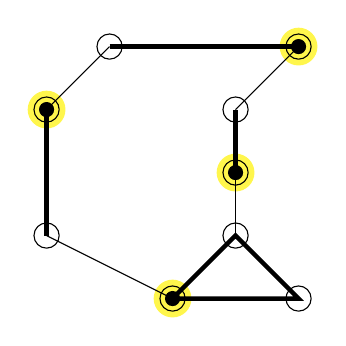
\begin{tikzpicture}[scale=0.8]
        \def\ver{0.12} %size of a vertex
        \def\xa{0}
        \def\ya{0}
        % Highlight change
        \draw[fill=yellow, opacity=.7, draw=none] (\xa-1,\ya-1)  circle (0.3cm);
        \draw[fill=yellow, opacity=.7, draw=none] (\xa-3,\ya+2) circle (0.3cm);
        \draw[fill=yellow, opacity=.7, draw=none] (\xa+1,\ya+3)  circle (0.3cm);
        \draw[fill=yellow, opacity=.7, draw=none] (\xa,\ya+1)  circle (0.3cm);

        %graph G
        \draw (\xa,\ya) circle (0.2cm);          % t11 no fill
        \draw (\xa+1,\ya-1) circle (0.2cm);      % t12 no fill
        \draw (\xa-1,\ya-1) circle (0.2cm);      % t13 no fill
        \draw (\xa-3,\ya) circle (0.2cm);        % e11 no fill
        \draw (\xa-3,\ya+2) circle (0.2cm);      % e12 no fill
        \draw (\xa-2,\ya+3) circle (0.2cm);      % e21 no fill
        \draw (\xa+1,\ya+3) circle (0.2cm);      % e22 no fill
        \draw (\xa,\ya+2) circle (0.2cm);        % e31 no fill
        \draw (\xa,\ya+1) circle (0.2cm);        % e32 no fill

        % Tokens
        \path[fill] (\xa-1,\ya-1) circle (\ver);   % t13
        \path[fill] (\xa-3,\ya+2) circle (\ver);   % e12
        \path[fill] (\xa+1,\ya+3) circle (\ver);   % e22
        \path[fill] (\xa,\ya+1) circle (\ver);     % e32

        % edges
        \draw[ultra thick] (\xa,\ya)--(\xa+1,\ya-1)--(\xa-1,\ya-1)--cycle;
        \draw[ultra thick] (\xa-3,\ya)--(\xa-3,\ya+2) ;
        \draw[ultra thick] (\xa-2,\ya+3)--(\xa+1,\ya+3) ;
        \draw[ultra thick] (\xa,\ya+2)--(\xa,\ya+1) ;

        \draw (\xa-2,\ya+3)--(\xa-3,\ya+2);
        \draw (\xa-3,\ya)--(\xa-1,\ya-1);
        \draw (\xa,\ya+1)--(\xa,\ya);
        \draw (\xa,\ya+2)--(\xa+1,\ya+3);

      \end{tikzpicture}
    \end{scaletikzpicturetowidth}
    \caption{An example of a restricted instance graph $G$ together with a standard token configuration.}
    \label{fig:standard_sliding}
\end{figure}


We say that a token configuration $T$ of $G_s$ is \textit{standard} if each token triangle and token edge of $G_s$ contains exactly one token
in $T$. Then, any move from a standard token configuration results in another standard token configuration since any token will never leave its
token triangle or token edge, and will never slide along a link edge because the first time any token would slide to another triangle or edge,
it would become adjacent to the token belonging to this triangle or edge. So tokens may never slide along a link edge. It is this latter
observation that will allow us to prove the $\PSPACE$-hardness of the labeled variant while doing only a little modification
in the original proof.

The sliding tokens problem remains $\PSPACE$-complete even if $G_s$ is such a restricted graph and both $T_0$ and $T_t$ are standard token
configurations \cite{bonsma}. This restricted problem is called the Standard sliding tokens problem.

\subsection{Labelled tokens} \label{subsection:coloring_problems}
In graph theory, graph coloring is a special case of graph labeling; it is an assignment of labels traditionally called "colors" to elements of a
graph subject to certain constraints. One of the simplest constraint is to color the vertices of a graph such that no two adjacent vertices
are of the same color, referred to as vertex colouring. Two prominent vertex coulouring problems that we will encounter and are part of the
hardness proof of the labelled sliding token problem are defined hereunder :

\subsubsection{$k$-colouring.}
For a positive integer $k$ and a graph $G$, we define the $k$-colour graph of $G$, denoted $\mathcal{C}_{k}(G)$,
as the graph that has the $k$-colourings of $G$ as its node set, with two $k$-colourings joined by an edge in $\mathcal{C}_{k}(G)$ if they differ
in colour on just one vertex of $G$. The $k$-COLOUR PATH is then defined as follows :
\begin{flushleft}
  k-COLOUR PATH \\
  \textbf{Instance: } Graph $G$, two $k$-colourings of $G, \alpha$ and $\beta$. \\
  \textbf{Question: } Is there a path between $\alpha$ and $\beta$ in $\mathcal{C}_{k}(G)$ ? \\
\end{flushleft}

\subsubsection{List colouring}
Suppose that we are given a graph $G=(V,E)$, and for each vertex of $G$, a list of colours permitted at that particular vertex.
In this context, the LIST-COLOUR PATH is defined as follows :
\begin{flushleft}
  LIST-COLOUR PATH \\
  \textbf{Instance: } Graph $G$, colour lists $L(v) \subseteq \{1,2,3,4\} \forall v \in V(G)$, two list-colourings $\alpha$ and $\beta$. \\
  \textbf{Question: } Is there a path between $\alpha$ and $\beta$ in $\mathcal{C}(G,L)$ ? \\
\end{flushleft}

An interesting relationship between the COLOUR-PATH problem and $k$-COLOUR PATH problem given by Bonsma is defined in lemma \ref{lemma:k_colour_to_list}.
\begin{lemma}\cite{bonsma}\label{lemma:k_colour_to_list}
For any $k \geq 4$, a LIST-COLOUR PATH instance $G, L, \alpha, \beta$ with lists $L(v) \subseteq \{1, 2, 3, 4\}$ can be transformed
into a $k$-COLOUR PATH instance $G^{'}, \alpha^{'}, \beta^{'}$ such that the distance between $\alpha$ and $\beta$ in $\mathcal{C}(G, L)$
(possibly infinite) is the same as the distance between $\alpha^{'}$ and $\beta^{'}$ in $\mathcal{C}_k(G^{'})$.
\end{lemma}

In \cite{bonsma}, Bonsma established that $k$-Colour Path is $\PSPACE$-complete for several graph classes and values of $k \geq 4$.
This result was obtained through a reduction from the Standard Sliding Token problem and done in two steps. First from the Standard
sliding token problem to the LIST-COLOUR path problem and then from the LIST-COLOUR path problem to the $k$-COLOUR path through lemma
\ref{lemma:k_colour_to_list}. In the following sections we will show that the hardness result remains even when the tokens in the
Standard sliding token instance are attributed unique labels.

\subsection{Preliminaries}
\paragraph{(a,b)-forbidding paths} For $a, b \in \{1, \dots, 4\}$,  an $(a, b)$-forbidding path from vertex $u$ to vertex $v$ is a
$(u, v)$-path with colour lists $L$, with $L(u), L(v) \neq \{1, 2, 3, 4\}$, such that in any colouring, it is not possible that
$u$ has colour $a$ and $v$ simultaneously has colour $b$ (please refer to \cite{bonsma} for the formal definition of (a,b)-forbidding paths).


\subsection{Reduction Structure}
Given a restricted instance $G, T_{A}, T_{B}, T$ of the Standard Sliding Token problem where $T$ is a set of labelled token (an example is
shown in figure \ref{fig:input_instance_standard}), we construct an instance $G^{'}, L, \alpha, \beta, T$ of LIST-COLOUR Path such that
standard token configurations of $G$ correspond to list-colourings of $G^{'}$ , and sliding a token in $G$ corresponds to a
sequence of vertex recolourings in $G^{'}$.

We first start by labelling the vertices of $G$: 
\begin{enumerate}
  \item The token triangles are labelled $1, \dots , n_{t}$ , and the vertices of each triangle $i$ are labelled
        $t_{i1}$, $t_{i2}$ and $t_{i3}$.
  \item The token edges are labelled $1, \dots , n_{e}$, and the vertices of each token edge $i$ are labelled
        $e_{i1}$ and $e_{i2}$.
\end{enumerate}

The construction of $G^{'}$ is as follows: For every token triangle $i$ in $G$ we introduce a vertex $t_{i}$, with colour list
$L(t_{i}) = \{1, 2, 3\}$ in $G^{'}$ . For every token edge $i$ in $G$ we introduce a vertex $e_{i}$ in $G^{'}$, with colour
list $L(e_{i}) = \{1, 2\}$. Whenever a link edge of $G$ joins a vertex $t_{ia}$ with a vertex $e_{jb}$, we add an $(a, b)$-forbidding
path of even length between $t_{i}$ and $e_{j}$ in $G$ . We do the same for pairs $t_{ia}$ and $t_{jb}$, and pairs $e_{ia}$ and $e_{jb}$.
Linking the vertices in $G^{'}$ through $(a, b)$-forbidding paths will make sure that no tokens are adjacent to each other (an example is
shown in figure \ref{fig:output_instance_standard}). Note that this is a polynomial-time transformation.

Standard token configurations of $G$ now correspond to colourings of $G^{'}$ as follows:
\begin{enumerate}
  \item For each token edge $i$ of the token configuration, the token being on $e_{ij} (j = 1, 2 )$
  corresponds to colourings of $G$ where $e_{i}$ has colour $j$.
  \item For each token triangle $i$ of the token configuration, the token being on $t_{ij} (j = 1, 2, 3)$,
  corresponds to colourings where $t_{i}$ has colour $j$.
\end{enumerate}

Since tokens are not adjacent, it is possible to choose colours for the internal vertices of the $(a, b)$-forbidding paths so as to
obtain a proper colouring of $G^{'}$. Two colourings $\alpha$ and $\beta$ corresponding to $T_{A}$ and $T_{B}$ respectively are constructed
this way. Note that to a given standard token configuration of $G$ there can correspond multiple colourings of $G$ because of the freedom
in choice of colours for the internal vertices of the $(a, b)$-forbidding paths.

For the labels, let $W$ be the set of token edges and token triangles of $G$ i.e., $W = \{e_1,\dots, e_{|E|} \} \cup \{t_1,\dots, t_{|T|} \}$
where $|E|$ is the total number of edge tokens in $G$ and $|T|$ is the total number of triangle tokens in $G$
and $f: T \rightarrow W$, a function mapping the set of given labels to the tokens on token edges and token triangles of $G$.

\begin{claim} Let $G, T_A, T_B$ be a restricted instance of Sliding Tokens where each token is given a unique label as described in
section \ref{sec:labeled_sliding_token}, and let $G , L, \alpha, \beta$ be the corresponding instance of List-Colour Path as constructed above.
Then $G, T_A, T_B$ is a Yes-instance if and only if $G , L, \alpha, \beta$ is a YES-instance.
\end{claim}\label{theorem:labeled_sliding}

\begin{proof} \cite{bonsma}
Recall that a token configuration in which the token of token edge $i$ (token triangle $i$) is on $e_{ij}$ (on $t_ {ij}$) corresponds
to multiple colourings of $G$ where $ei$ ($t_i$) has colour $j$. Because of this multiplicity of colourings, we define colour classes of
colourings: if two colourings $\kappa$ and $\lambda$ of $G$ have $\kappa(t_i) = \lambda(t_i)$ and $\kappa(e_i) = \lambda(e_i)$ for every $i$,
then $\kappa$ and $\lambda$ are said to be in the same colour class.

Hence the correspondence between standard token configurations and colourings defines a mapping between standard
token configurations and colour classes. This mapping is in fact a bijection: $(a, b)$-forbidding paths restrict their end vertices
from having colours $a$ and $b$ respectively, but they pose no other restriction on the possible colours of their end vertices.
So $t_{ia}$ and $e_{jb}$ cannot both be occupied by a token in a token configuration if and only if no colouring $\kappa$ has $\kappa(t_i)$ = $a$
and $\kappa(e_j) = b$. (Similar statements hold for pairs $t_i$ and $t_j$, and pairs $e_i$ and $e_j$.)

The function $f$ also yields a bijective mapping : Since no token can slide along a link edge in the Standard sliding token,
each element $w \in W$ can be attributed a label such that the colour of $w$ in the output LIST-COULOUR path instance represents
the vertex placement of the label $t \in T$ s.t $f(t) = w$.

Now we claim that if there exists a sequence of moves that transforms $T_A$ into $T_B$, then there exists a sequence of
recolourings that transforms $\alpha$ into $\beta$. We mentioned earlier that any token configuration obtainable from $T_A$ is a standard
token configuration \cite{bonsma}. Hence every token move corresponds to recolouring a vertex $t_i$ or a vertex $e_i$. Note that before
recolouring $t_i$ (or $e_i$), it may be necessary to first recolour some internal vertices of $(a, b)$-forbidding paths incident with
$t_i$ (or $e_i$), but by the definition of $(a, b)$-forbidding paths, we know this is always possible. It can also be seen that when
we finally arrive in the colour class that contains $\beta$ in this way, the internal vertices of all $(a, b)$-forbidding paths can be
recoloured so that exactly the colouring $\beta$ is obtained.

Similarly, for every sequence of recolourings from $\alpha$ to $\beta$ we can construct a sequence of token moves from $T_A$ to $T_B$:
whenever a vertex $t_i$ ($e_i$) is recoloured from colour a to colour $b$, we move the corresponding token from $t_{ia}$ to $t_{ib}$
(from $e_ {ia}$ to $e_{ib}$). This completes the proof.
\end{proof}

\begin{example}{STANDARD SLIDING TOKEN problem to COLOUR-PATH reduction. \\}
  \textbf{Instance instance : STANDARD SLIDING TOKEN instance.} \hfill

\begin{figure}[H]
  \centering
  \begin{subfigure}[b]{0.4\textwidth}
    \begin{scaletikzpicturetowidth}{\textwidth}
      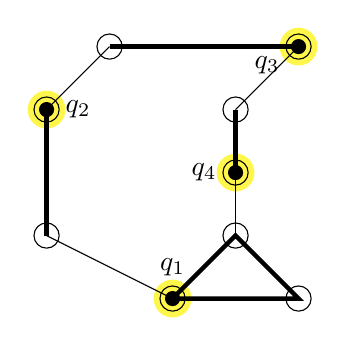
\begin{tikzpicture}[scale=0.8]
        \def\ver{0.12} %size of a vertex
        \def\xa{0}
        \def\ya{0}
        % Highlight change
        \draw[fill=yellow, opacity=.7, draw=none] (\xa-1,\ya-1)  circle (0.3cm);
        \draw[fill=yellow, opacity=.7, draw=none] (\xa-3,\ya+2) circle (0.3cm);
        \draw[fill=yellow, opacity=.7, draw=none] (\xa+1,\ya+3)  circle (0.3cm);
        \draw[fill=yellow, opacity=.7, draw=none] (\xa,\ya+1)  circle (0.3cm);
        %graph G
        \draw (\xa,\ya) circle (0.2cm);          % t11 no fill
        \draw (\xa+1,\ya-1) circle (0.2cm);      % t12 no fill
        \draw (\xa-1,\ya-1) circle (0.2cm);      % t13 no fill
        \draw (\xa-3,\ya) circle (0.2cm);        % e11 no fill
        \draw (\xa-3,\ya+2) circle (0.2cm);      % e12 no fill
        \draw (\xa-2,\ya+3) circle (0.2cm);      % e21 no fill
        \draw (\xa+1,\ya+3) circle (0.2cm);      % e22 no fill
        \draw (\xa,\ya+2) circle (0.2cm);        % e31 no fill
        \draw (\xa,\ya+1) circle (0.2cm);        % e32 no fill
        % Tokens
        \path[fill] (\xa-1,\ya-1) circle (\ver);   % t13
        \path[fill] (\xa-3,\ya+2) circle (\ver);   % e12
        \path[fill] (\xa+1,\ya+3) circle (\ver);   % e22
        \path[fill] (\xa,\ya+1) circle (\ver);     % e32
        % edges
        \draw[ultra thick] (\xa,\ya)--(\xa+1,\ya-1)--(\xa-1,\ya-1)--cycle;
        \draw[ultra thick] (\xa-3,\ya)--(\xa-3,\ya+2) ;
        \draw[ultra thick] (\xa-2,\ya+3)--(\xa+1,\ya+3) ;
        \draw[ultra thick] (\xa,\ya+2)--(\xa,\ya+1) ;
        \draw (\xa-2,\ya+3)--(\xa-3,\ya+2);
        \draw (\xa-3,\ya)--(\xa-1,\ya-1);
        \draw (\xa,\ya+1)--(\xa,\ya);
        \draw (\xa,\ya+2)--(\xa+1,\ya+3);
        % token labels
        \node (l1) at (\xa-1,\ya-0.5) {$q_{1}$};            % Label
        \node (l2) at (\xa-2.5,\ya+2) {$q_{2}$};            % Label
        \node (l3) at (\xa+0.5,\ya+2.7) {$q_{3}$};            % Label
        \node (l4) at (\xa-0.5,\ya+1) {$q_{4}$};            % Label

      \end{tikzpicture}
    \end{scaletikzpicturetowidth}
    \caption{Initial token configuration $T_{A}$.}
    \label{fig:standard_1}
  \end{subfigure}
  \begin{subfigure}[b]{0.4\textwidth}
    \begin{scaletikzpicturetowidth}{\textwidth}
      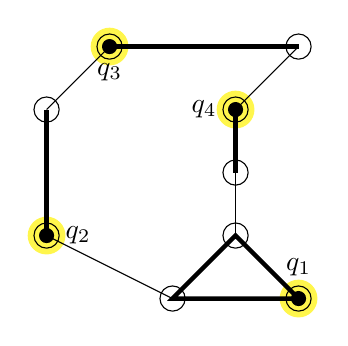
\begin{tikzpicture}[scale=0.8]
        \def\ver{0.12} %size of a vertex
        \def\xa{0}
        \def\ya{0}
        % Highlight change
        \draw[fill=yellow, opacity=.7, draw=none] (\xa+1,\ya-1)  circle (0.3cm);
        \draw[fill=yellow, opacity=.7, draw=none] (\xa-3,\ya) circle (0.3cm);
        \draw[fill=yellow, opacity=.7, draw=none] (\xa-2,\ya+3)  circle (0.3cm);
        \draw[fill=yellow, opacity=.7, draw=none] (\xa,\ya+2)  circle (0.3cm);
        %graph G
        \draw (\xa,\ya) circle (0.2cm);          % t11 no fill
        \draw (\xa+1,\ya-1) circle (0.2cm);      % t12 no fill
        \draw (\xa-1,\ya-1) circle (0.2cm);      % t13 no fill
        \draw (\xa-3,\ya) circle (0.2cm);        % e11 no fill
        \draw (\xa-3,\ya+2) circle (0.2cm);      % e12 no fill
        \draw (\xa-2,\ya+3) circle (0.2cm);      % e21 no fill
        \draw (\xa+1,\ya+3) circle (0.2cm);      % e22 no fill
        \draw (\xa,\ya+2) circle (0.2cm);        % e31 no fill
        \draw (\xa,\ya+1) circle (0.2cm);        % e32 no fill
        % Tokens
        \path[fill] (\xa+1,\ya-1) circle (\ver);   % t12
        \path[fill] (\xa-3,\ya) circle (\ver);     % e11
        \path[fill] (\xa-2,\ya+3) circle (\ver);   % e21
        \path[fill] (\xa,\ya+2) circle (\ver);     % e31
        % edges
        \draw[ultra thick] (\xa,\ya)--(\xa+1,\ya-1)--(\xa-1,\ya-1)--cycle;
        \draw[ultra thick] (\xa-3,\ya)--(\xa-3,\ya+2) ;
        \draw[ultra thick] (\xa-2,\ya+3)--(\xa+1,\ya+3) ;
        \draw[ultra thick] (\xa,\ya+2)--(\xa,\ya+1) ;
        \draw (\xa-2,\ya+3)--(\xa-3,\ya+2);
        \draw (\xa-3,\ya)--(\xa-1,\ya-1);
        \draw (\xa,\ya+1)--(\xa,\ya);
        \draw (\xa,\ya+2)--(\xa+1,\ya+3);
        % token labels
        \node (l1) at (\xa+1,\ya-0.5) {$q_{1}$};            % Label (\xa+1,\ya-1)
        \node (l2) at (\xa-2.5,\ya) {$q_{2}$};            % Label (\xa-3,\ya)
        \node (l3) at (\xa-2,\ya+2.6) {$q_{3}$};            % Label (\xa-2,\ya+3)
        \node (l4) at (\xa-0.5,\ya+2) {$q_{4}$};            % Label (\xa,\ya+2)
      \end{tikzpicture}
    \end{scaletikzpicturetowidth}
    \caption{Target token configuration $T_{B}$.}
    \label{fig:standard_2}
  \end{subfigure}
  \caption{A Standard sliding token instance with initial and target labelled token configuration $T_{A}$ and $T_{B}$ respectively.}
  \label{fig:input_instance_standard}
\end{figure}

% ------------------------- Output instance 1 -----------------------------
  \textbf{Output instance : LIST-COLOUR path instance.} \hfill
\begin{figure}[H]
  \begin{subfigure}[b]{0.9\textwidth}
    \begin{scaletikzpicturetowidth}{\textwidth}
      \begin{tikzpicture}[scale=0.8]
        \centering
        \def\ver{0.12} %size of a vertex
        \def\xa{0}
        \def\ya{0}
        \node[Bullet=purple,label=above :{$\{1,2,3\}$}] (t1) at (\xa,\ya+3){};             % t1
        \node[Bullet=blue,label=left :{$\{1,3\}$}] (t11) at (\xa-3,\ya+1.5){};             % t11
        \node[Bullet=blue,label=right:{$\{2,1\}$}] (e33) at (\xa+1.5,\ya+2.2){};           % e33
        \node[Bullet=green,label=right:{$\{2,3\}$}] (e32) at (\xa+3,\ya+1.5){};            % e32
        \node[Bullet=purple,label=right:{$\{3,2\}$}] (e31) at (\xa+4.5,\ya+0.8){};         % e31
        \node[Bullet=green,label=below :{$\{1,2\}$}] (e3) at (\xa+6,\ya){};                % e3
        \node[Bullet=blue,label=below :{$\{3,1\}$}] (e23) at (\xa+4.5,\ya){};              % e23
        \node[Bullet=purple,label=below :{$\{1,3\}$}] (e22) at (\xa+3,\ya){};              % e22
        \node[Bullet=blue,label=below :{$\{1,2\}$}] (e21) at (\xa+1.5,\ya){};              % e21
        \node[Bullet=green,label=above :{$\{1,2\}$}] (e2) at (\xa,\ya){};                  % e2
        \node[Bullet=blue,label=below :{$\{3,1\}$}] (e13) at (\xa-1.5,\ya){};              % e13
        \node[Bullet=purple,label=below :{$\{1,3\}$}] (e12) at (\xa-3,\ya){};              % e12
        \node[Bullet=blue,label=below :{$\{1,2\}$}] (e11) at (\xa-4.5,\ya){};              % e11
        \node[Bullet=green,label=below :{$\{1,2\}$}] (e1) at (\xa-6,\ya){};                % e1

        \draw[thick] (e1)--(e11)--(e12)--(e13)--(e2)--(e21)--(e22)--(e23)--(e3)--(e31)--(e32)--(e33)--(t1)--(t11)--(e1);
      \end{tikzpicture}
    \end{scaletikzpicturetowidth}
    \caption{Initial colouring $\alpha$.}
    \label{fig:list_colour_1}
  \end{subfigure}
  \medskip
  \begin{subfigure}[b]{0.9\textwidth}
    \begin{scaletikzpicturetowidth}{\textwidth}
      \begin{tikzpicture}[scale=0.8]
        \centering
        \def\ver{0.12} %size of a vertex
        \def\xa{0}
        \def\ya{0}
        \node[Bullet=green,label=above :{$\{1,2,3\}$}] (t1) at (\xa,\ya+3){};             % t1
        \node[Bullet=purple,label=left :{$\{1,3\}$}] (t11) at (\xa-3,\ya+1.5){};          % t11
        \node[Bullet=blue,label=right:{$\{2,1\}$}] (e33) at (\xa+1.5,\ya+2.2){};          % e33
        \node[Bullet=green,label=right:{$\{2,3\}$}] (e32) at (\xa+3,\ya+1.5){};           % e32
        \node[Bullet=purple,label=right:{$\{3,2\}$}] (e31) at (\xa+4.5,\ya+0.8){};        % e31
        \node[Bullet=blue,label=below :{$\{1,2\}$}] (e3) at (\xa+6,\ya){};                % e3
        \node[Bullet=purple,label=below :{$\{3,1\}$}] (e23) at (\xa+4.5,\ya){};           % e23
        \node[Bullet=blue,label=below :{$\{1,3\}$}] (e22) at (\xa+3,\ya){};               % e22
        \node[Bullet=green,label=below :{$\{1,2\}$}] (e21) at (\xa+1.5,\ya){};            % e21
        \node[Bullet=blue,label=above :{$\{1,2\}$}] (e2) at (\xa,\ya){};                  % e2
        \node[Bullet=purple,label=below :{$\{3,1\}$}] (e13) at (\xa-1.5,\ya){};           % e13
        \node[Bullet=blue,label=below :{$\{1,3\}$}] (e12) at (\xa-3,\ya){};               % e12
        \node[Bullet=green,label=below :{$\{1,2\}$}] (e11) at (\xa-4.5,\ya){};            % e11
        \node[Bullet=blue,label=below :{$\{1,2\}$}] (e1) at (\xa-6,\ya){};                % e1

        \draw[thick] (e1)--(e11)--(e12)--(e13)--(e2)--(e21)--(e22)--(e23)--(e3)--(e31)--(e32)--(e33)--(t1)--(t11)--(e1);
      \end{tikzpicture}
    \end{scaletikzpicturetowidth}
    \caption{Target colouring $\beta$}
    \label{fig:list_colour_2}
  \end{subfigure}
  \caption{Output LIST-COLOUR path instance with $\alpha$ being the initial colouring and $\beta$ the target colouring where for better
  visualisation the colour blue is associated to 1, green to 2 and purple to 3 .}
  \label{fig:output_instance_standard}
\end{figure}
\end{example}